\chapter{Proof of concept}
\label{ch:proofofconcept}
Dit hoofdstuk bevat de proof of concept die voor Dropsolid werd uitgewerkt. Dit is een \gls{testsuite} die met Nightwatch gemaakt is om de \gls{Paragraph Types} op Rocketship, de Drupal 8 installatie van Dropsolid, te testen. In dit hoofdstuk wordt eerst uitgelegd wat Rocketship is en wat de verschillende \gls{Paragraph Types} zijn. Hierna wordt de installatie en configuratie van Nightwatch besproken. Vervolgens wordt de code van de testen opgelijst en wordt uigelegd wat er specifiek in de test gebeurt. Ten slotte wordt de code van de verschillende commando's die voor de testen werd geschreven opgelijst en toegelicht.

\clearpage
\section{Rocketship \& Paragraph Types}
Rocketship is het installatieprofiel van Drupal dat Dropsolid heeft ontwikkeld. Dit wil zeggen dat er na de installatie van Rocketship, een werkende versie van een Drupal 8 site beschikbaar is die al voorgeprogrammeerde zaken bevat om het ontwikkelingsproces van een website te versnellen en vereenvoudigen.

\gls{Paragraph Types} zijn voorgeprogrammeerde blokken die aan een website kunnen toegevoegd worden. Dit zijn bijvoorbeeld blokken waarin een afbeelding kan geplaatst worden of blokken die een titel en wat tekst bevatten.

\clearpage
\subsection{Paragraph 1: Story}
De eerste Paragraph is een blok met een titel, een subtitel, een tekstveld, een afbeelding en een button die linkt naar een andere pagina.
\begin{figure}[h]
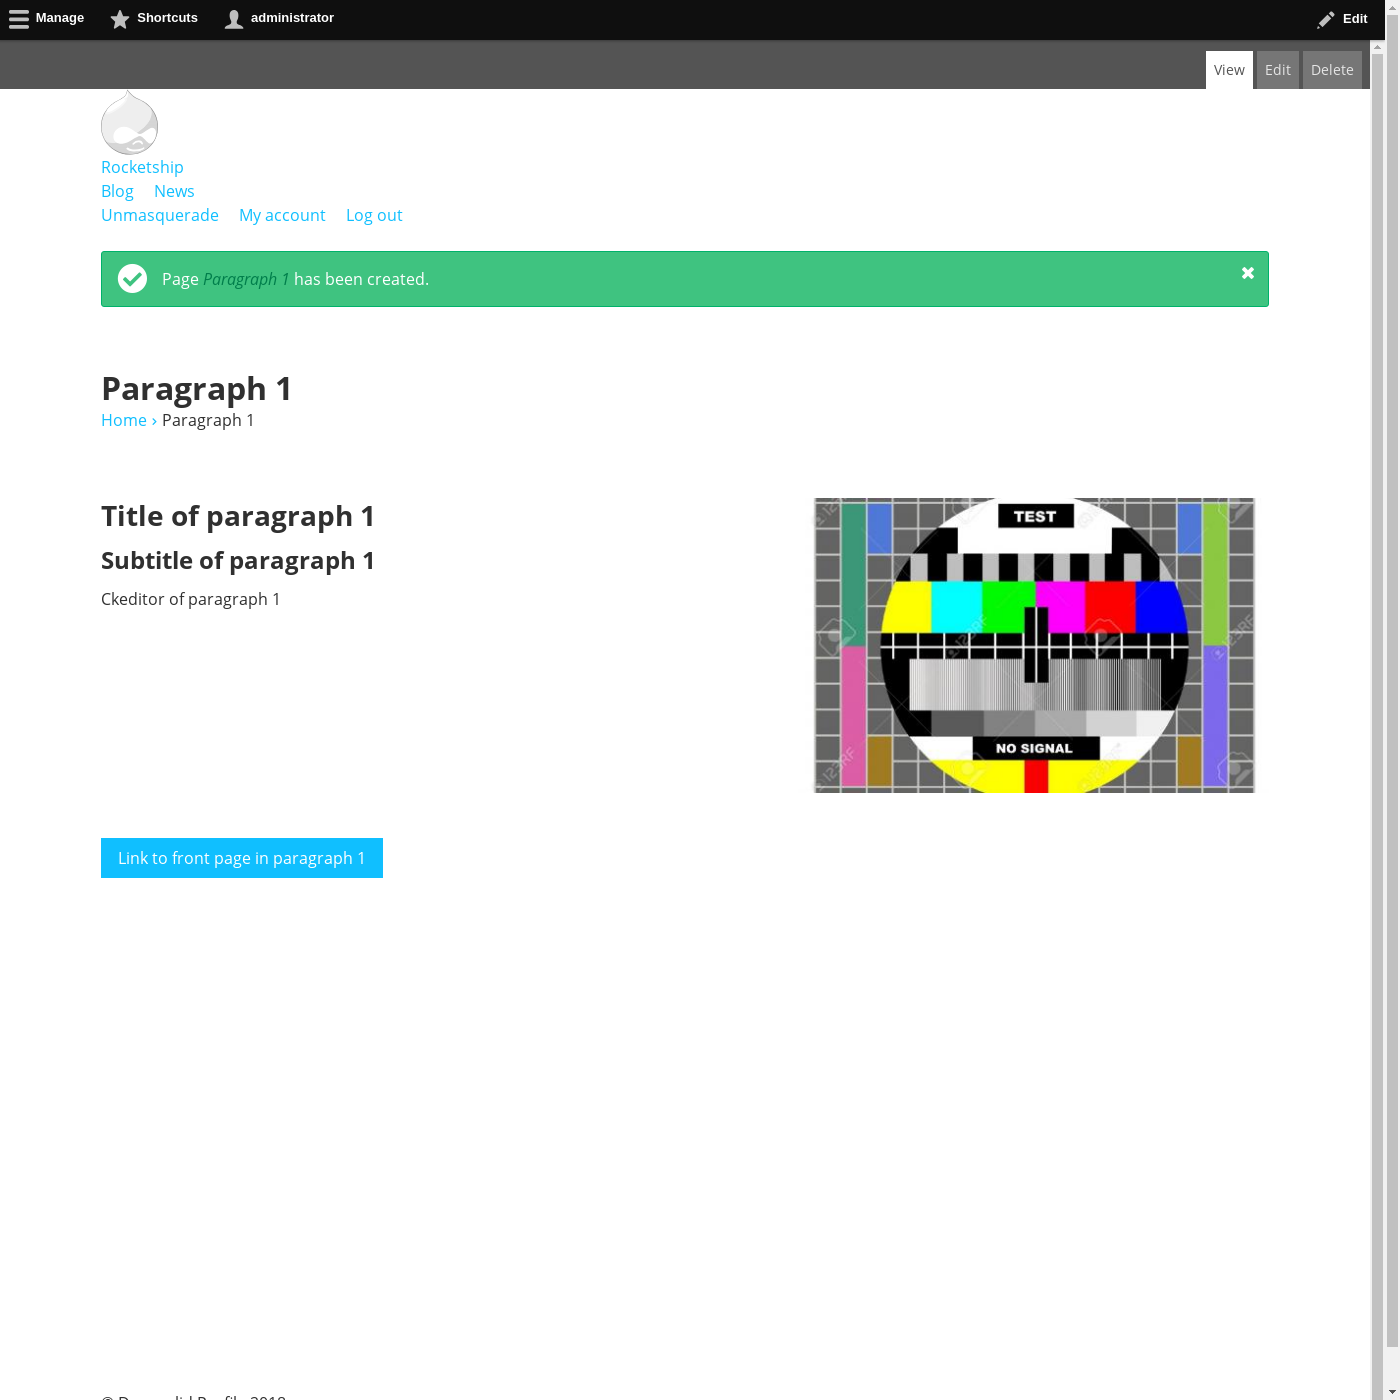
\includegraphics[width=1\textwidth]{img/p001.png}
\end{figure}

\clearpage
\subsection{Paragraph 2: Image}
De tweede Paragraph is een blok die een afbeelding bevat en linkt naar een andere pagina.
\begin{figure}[h]
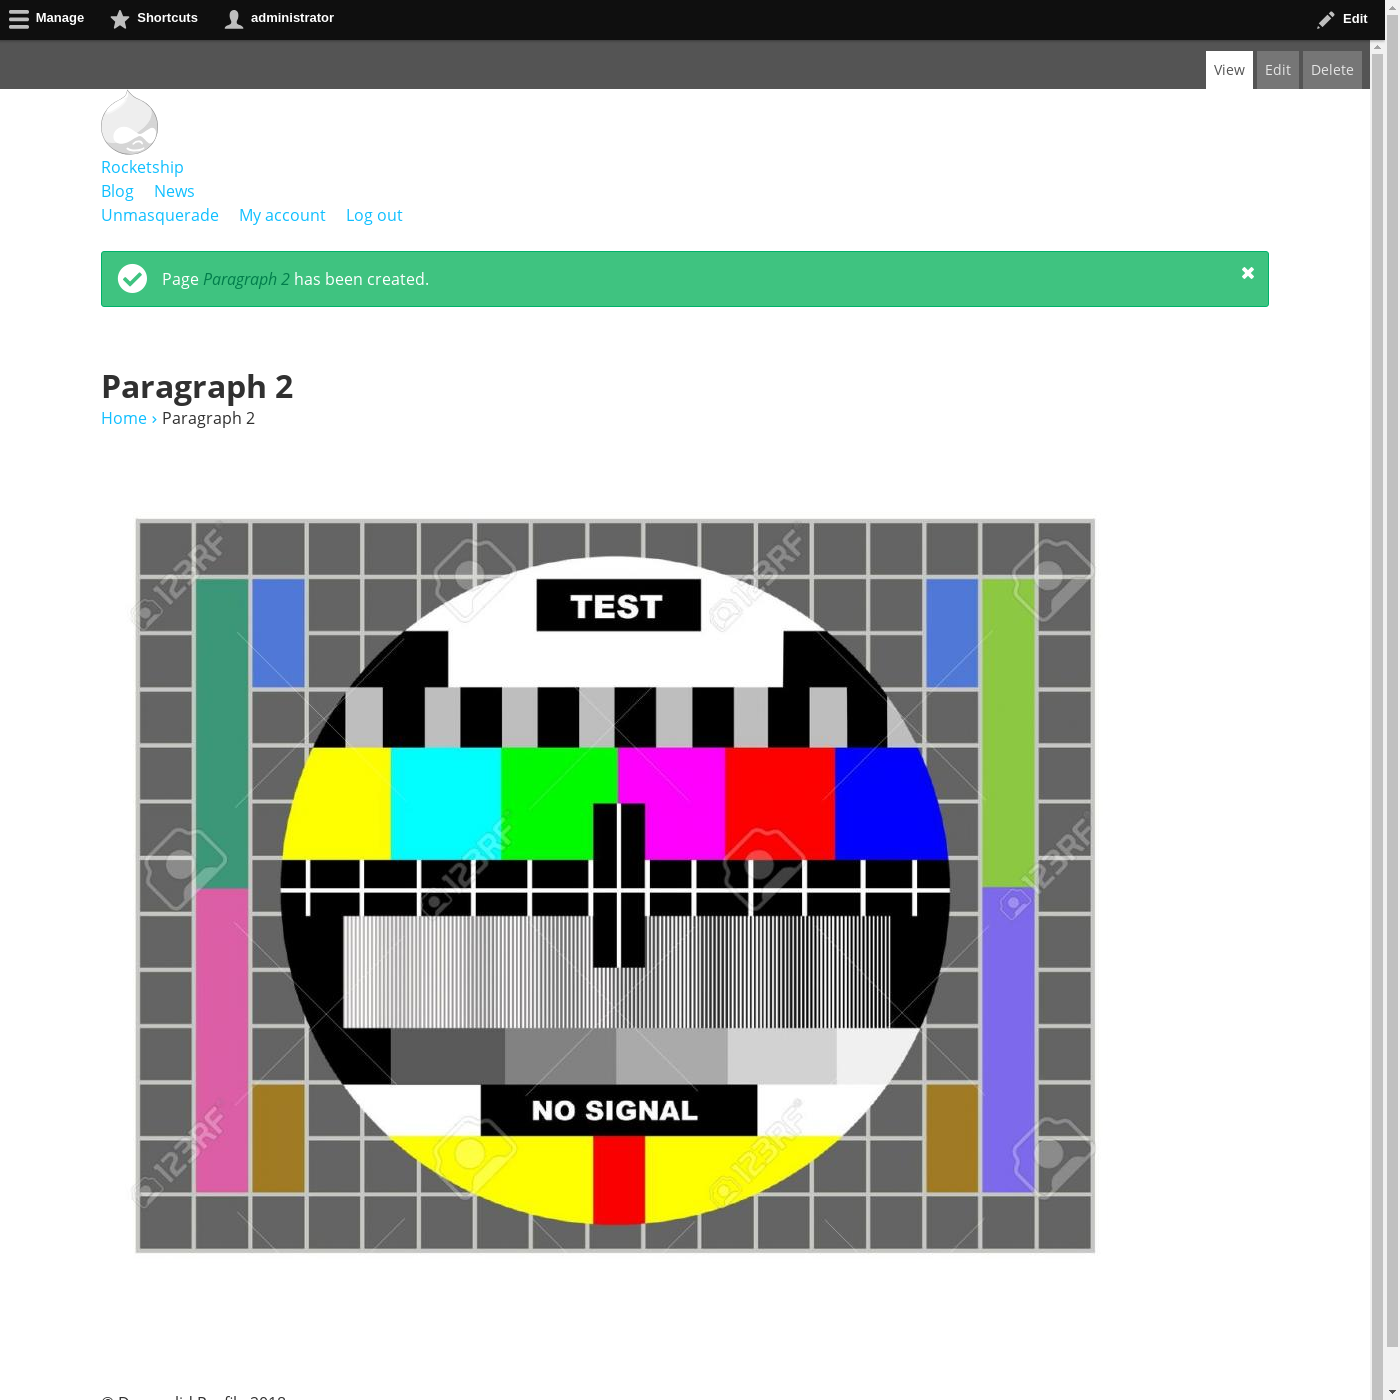
\includegraphics[width=1\textwidth]{img/p002.png}
\end{figure}

\clearpage
\subsection{Paragraph 3: Text main}
De derde Paragraph is een blok met een titel, een teaser, een tekstveld en een button die linkt naar een andere pagina.
\begin{figure}[h]
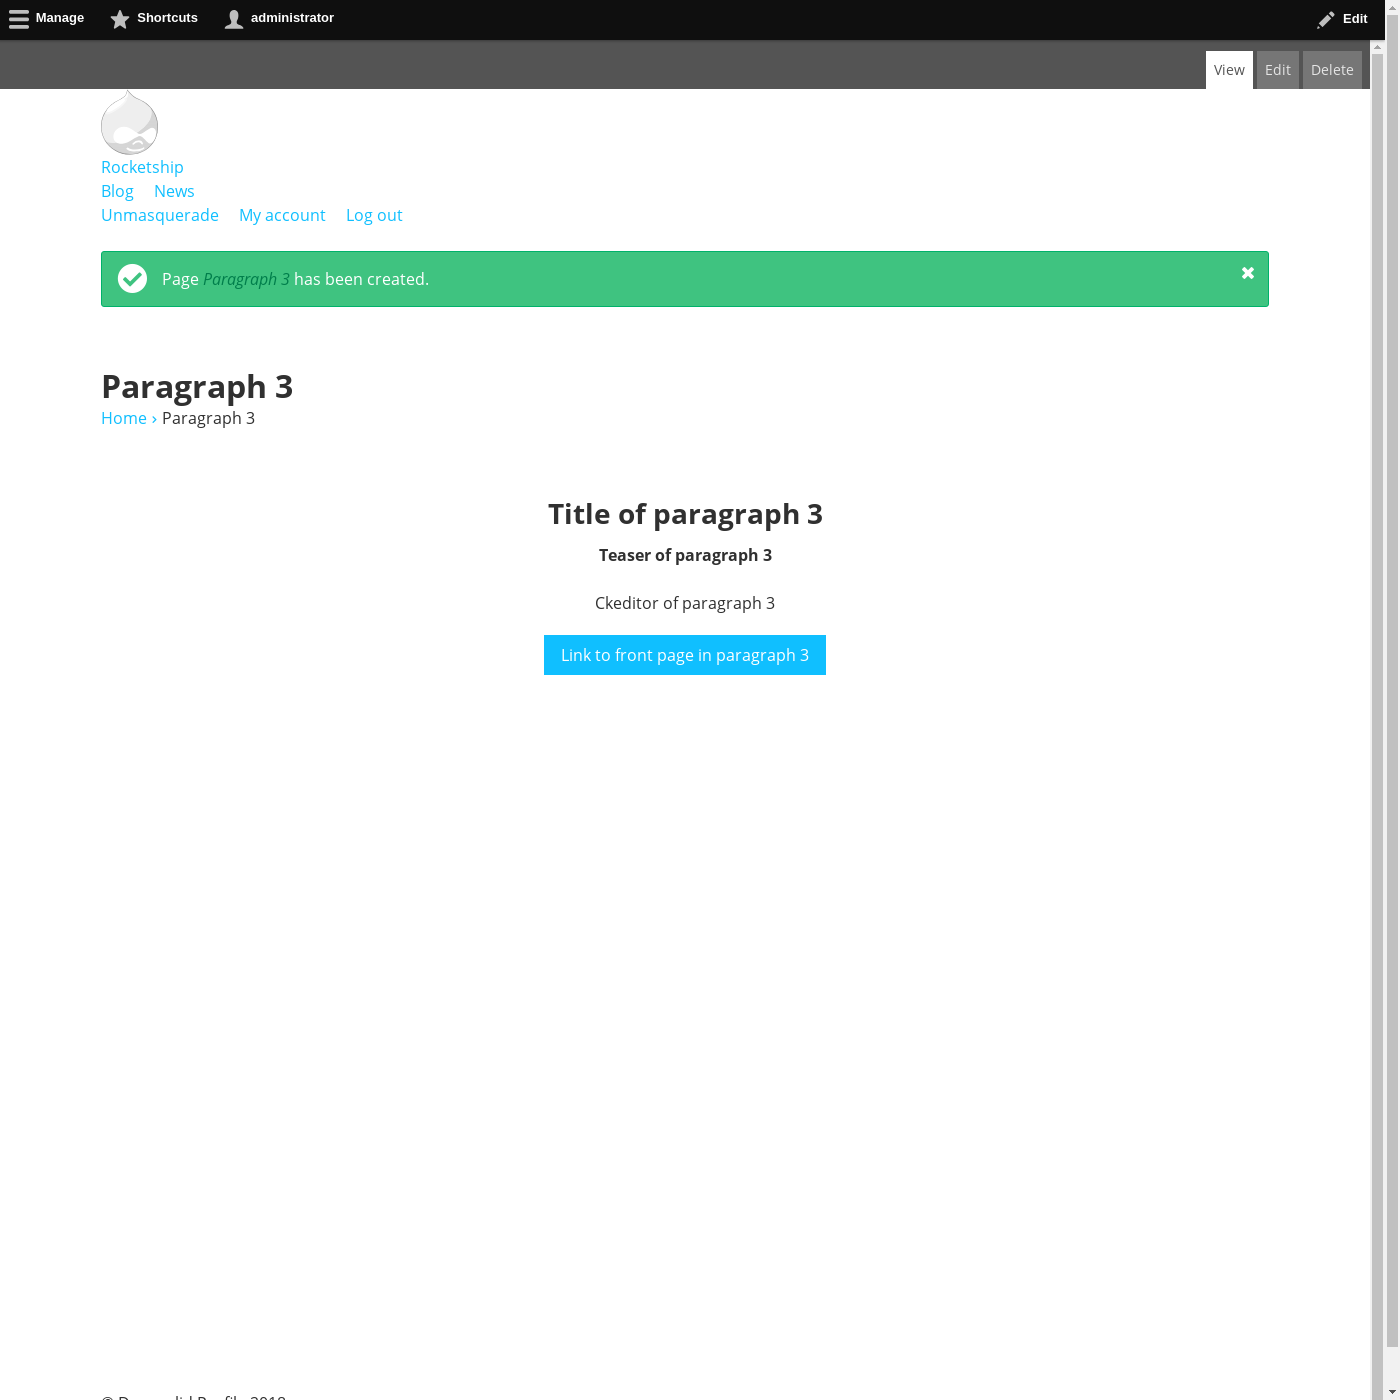
\includegraphics[width=1\textwidth]{img/p003.png}
\end{figure}

\clearpage
\subsection{Paragraph 4: FAQ}
De vierde Paragraph is een blok met een titel, een subtitel en een teaser met daaronder veelgestgestelde vragen die kunnen open geklikt worden om het antwoord er op te zien.
\begin{figure}[h]
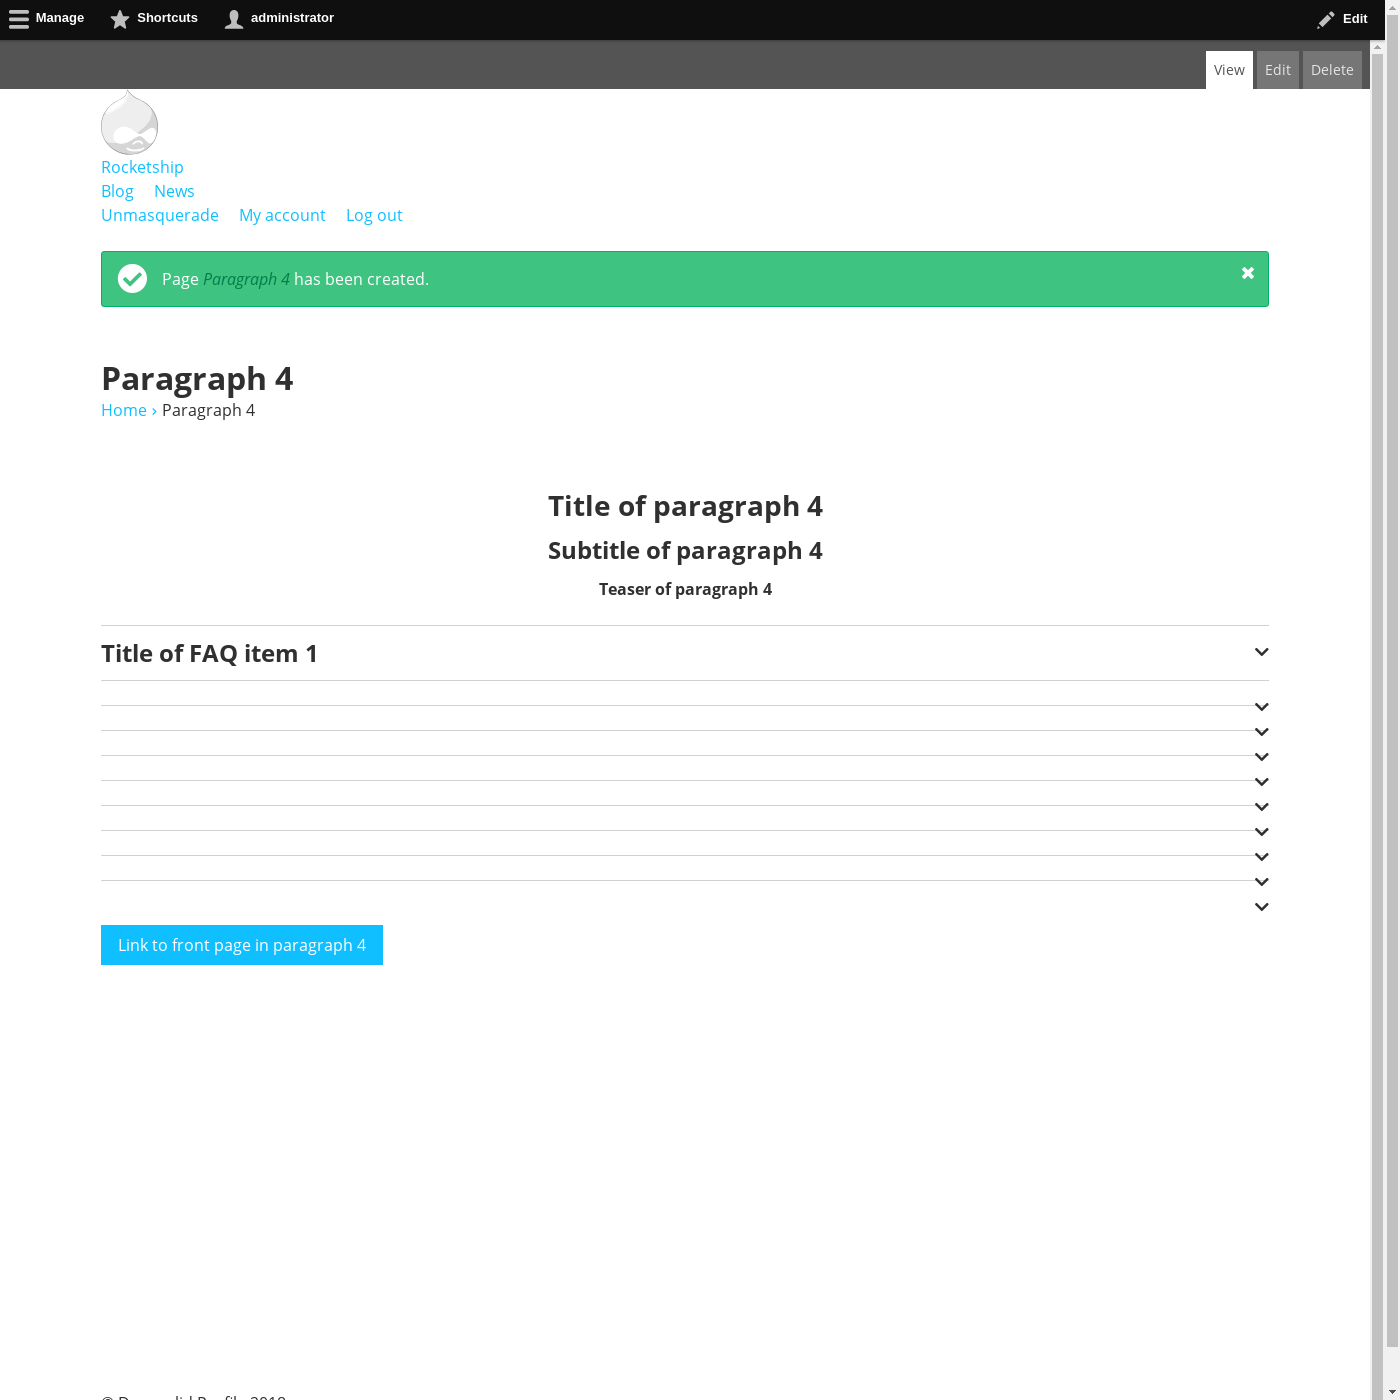
\includegraphics[width=1\textwidth]{img/p004.png}
\end{figure}

\clearpage
\subsection{Paragraph 5: Testimonial}
De vijfde Paragraph is een blok die een afbeelding, een quote, een  naam, een extra tekstveld en een link naar een andere pagina bevat.
\begin{figure}[h]
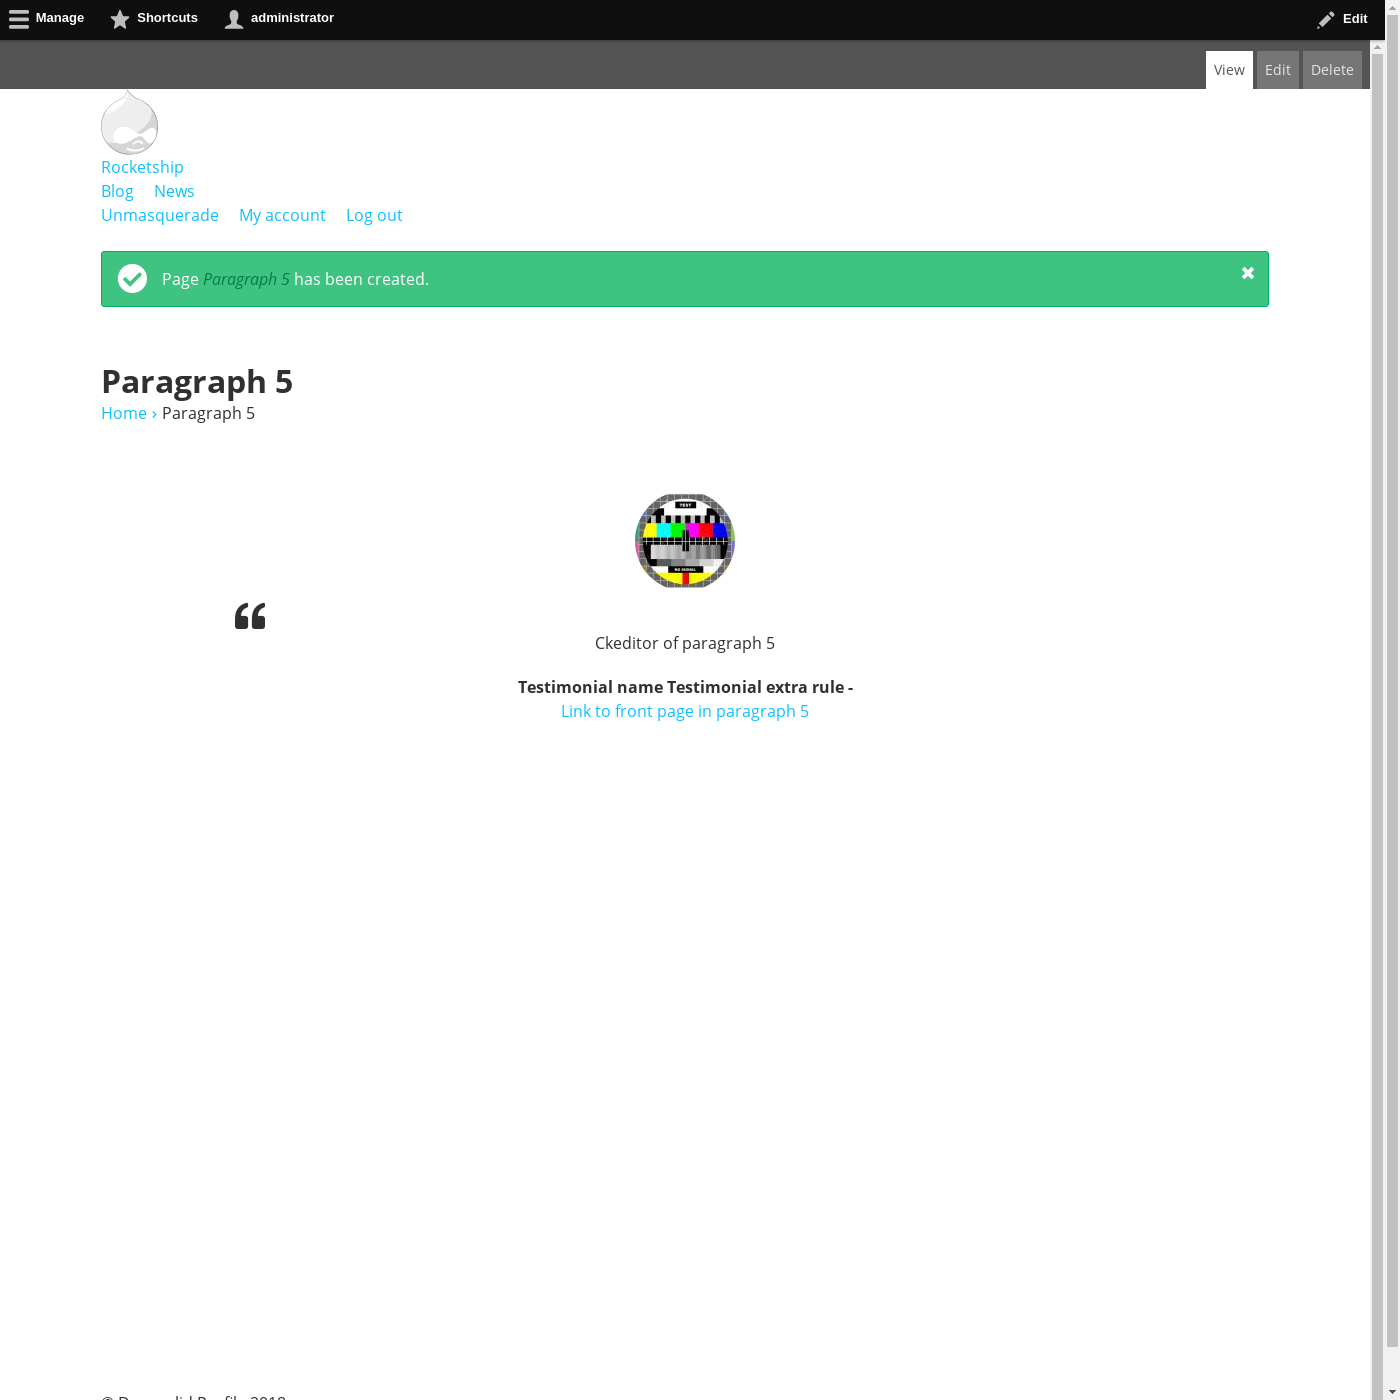
\includegraphics[width=1\textwidth]{img/p005.png}
\end{figure}

\clearpage
\subsection{Paragraph 6: Video}
De zesde Paragraph is een blok die een Youtube of Vimeo video bevat.
\begin{figure}[h]
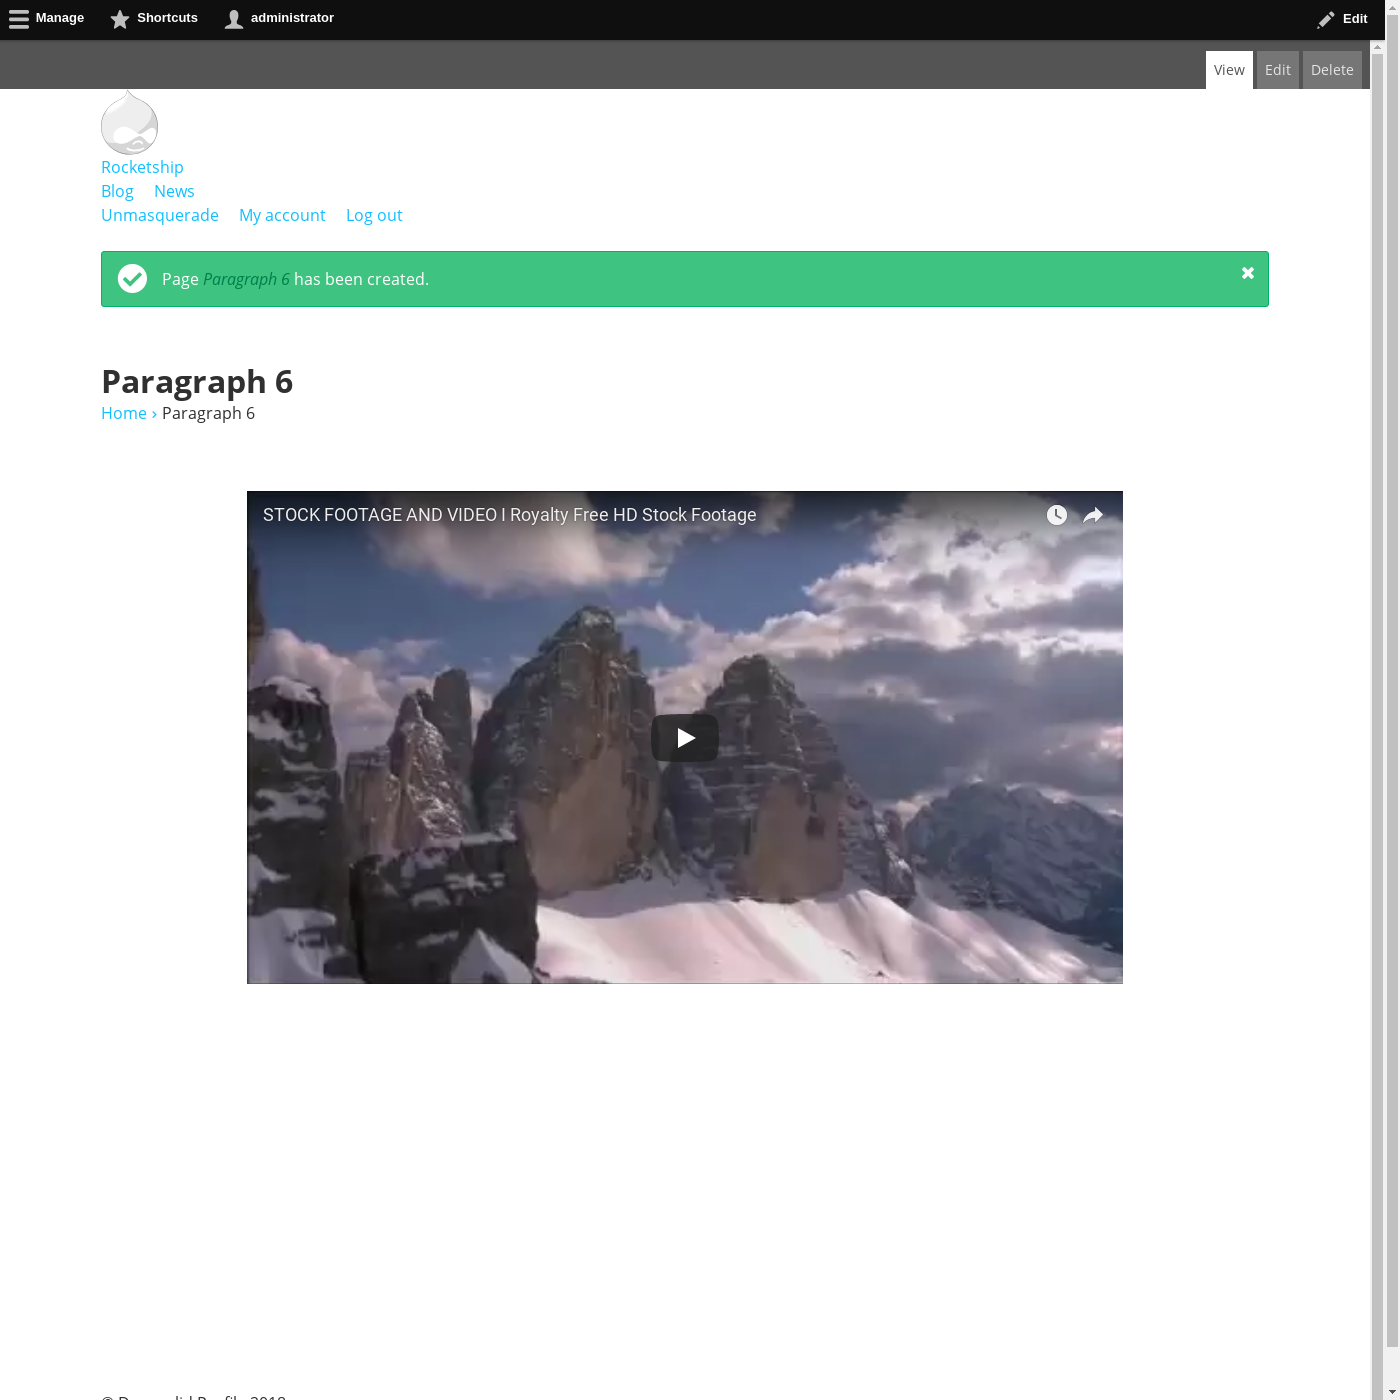
\includegraphics[width=1\textwidth]{img/p006.png}
\end{figure}

\clearpage
\subsection{Paragraph 7: USP}
De zevende Paragraph is een blok met een titel, subtitel en teaser. Hieronder staat een USP item dat een afbeelding, titel en tekstveld bevat. Onder de USP items staat er ook nog eens een button die linkt naar een andere pagina.
\begin{figure}[h]
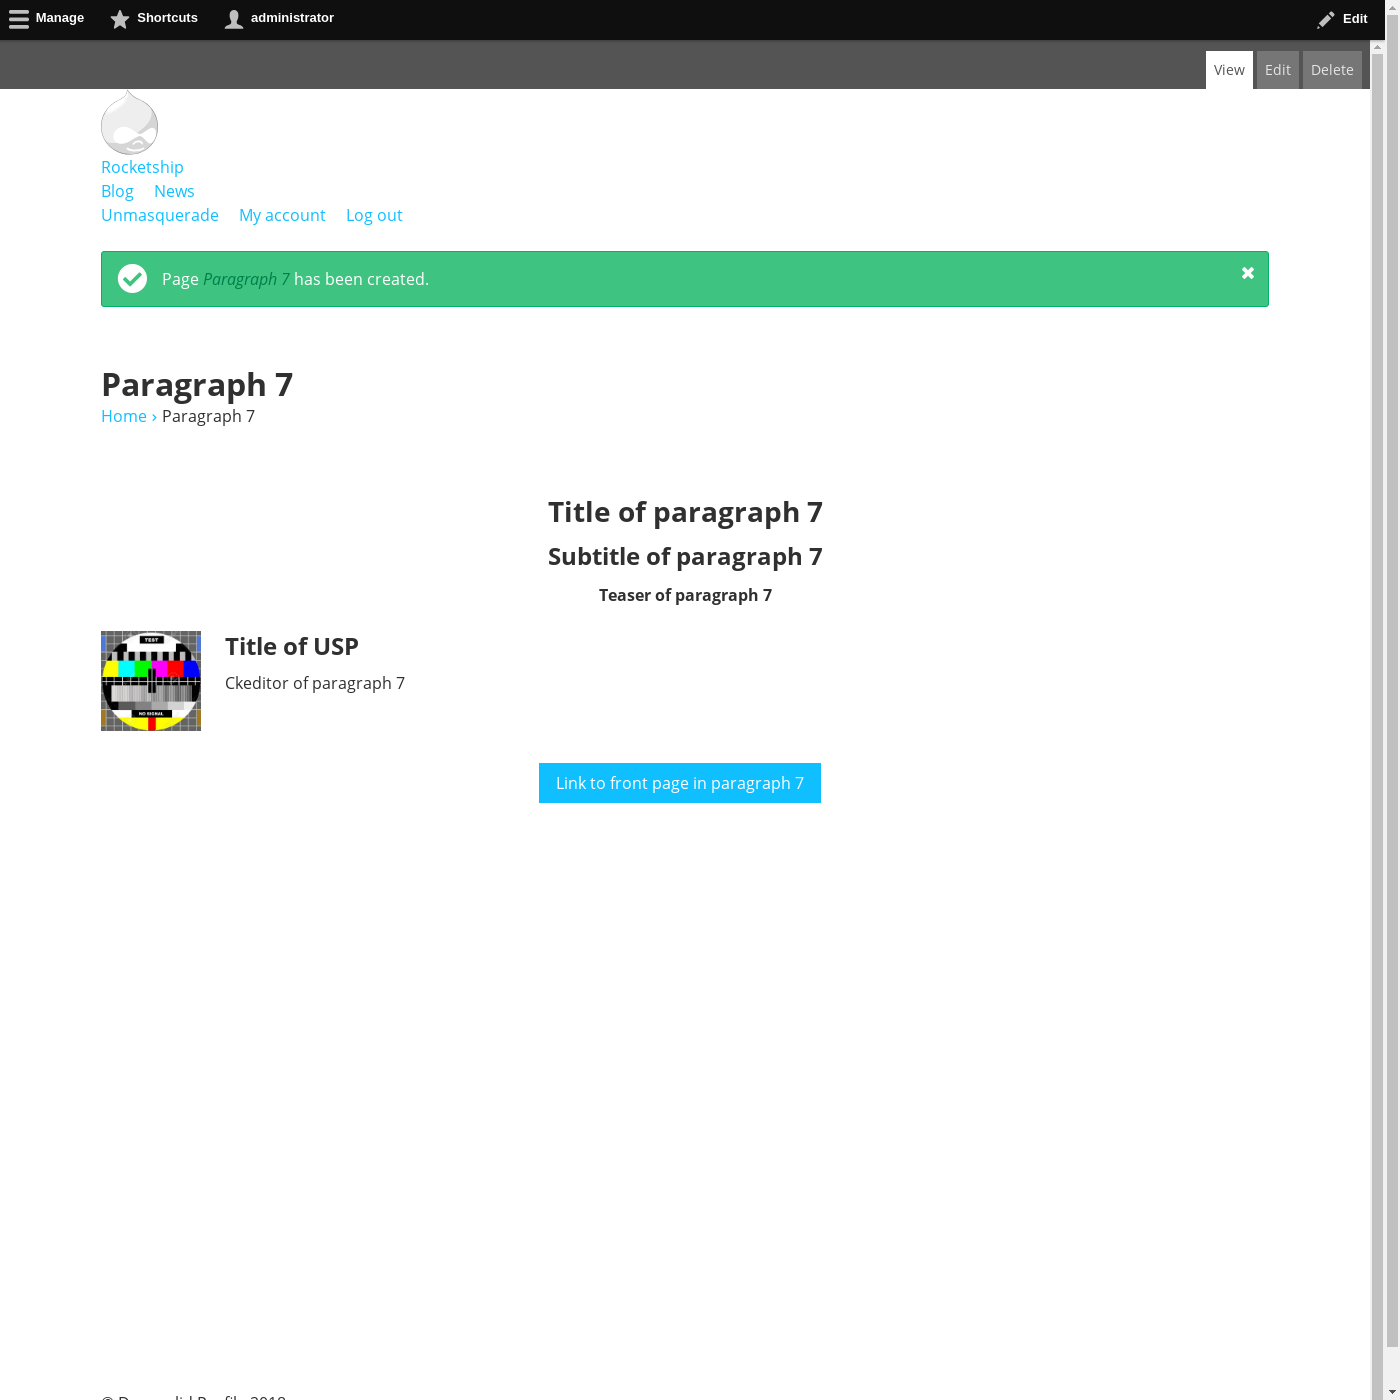
\includegraphics[width=1\textwidth]{img/p007.png}
\end{figure}

\clearpage
\subsection{Paragraph 8: Focus}
De achtste Paragraph is gelijkaardig aan de derde Paragraph en is een blok met een titel, subtitel, teaser en button die linkt naar een andere pagina.
\begin{figure}[h]
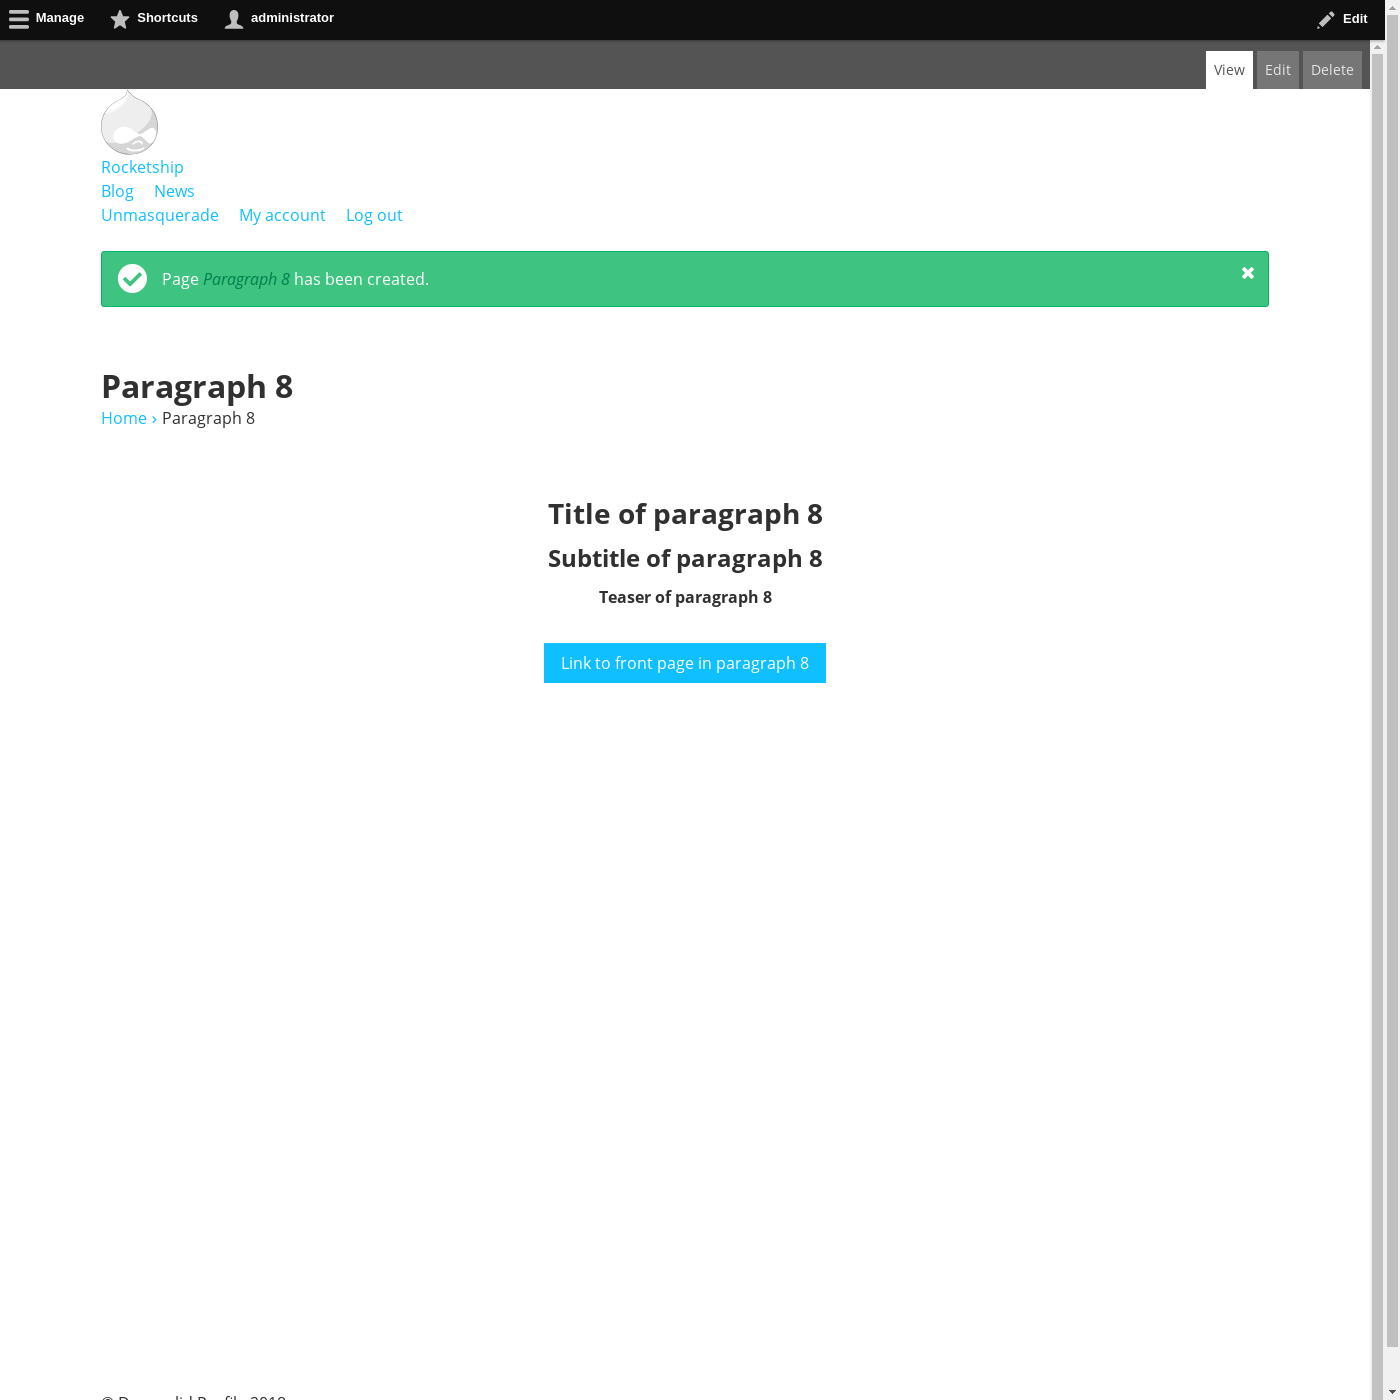
\includegraphics[width=1\textwidth]{img/p008.png}
\end{figure}

\clearpage
\subsection{Paragraph 9: Photo gallery}
De negende Paragraph is een blok met een titel, subtitel en teaser. Hieronder staan afbeeldingen die linken naar een andere pagina en de blok wordt afgesloten met een button die ook een link bevat.
\begin{figure}[h]
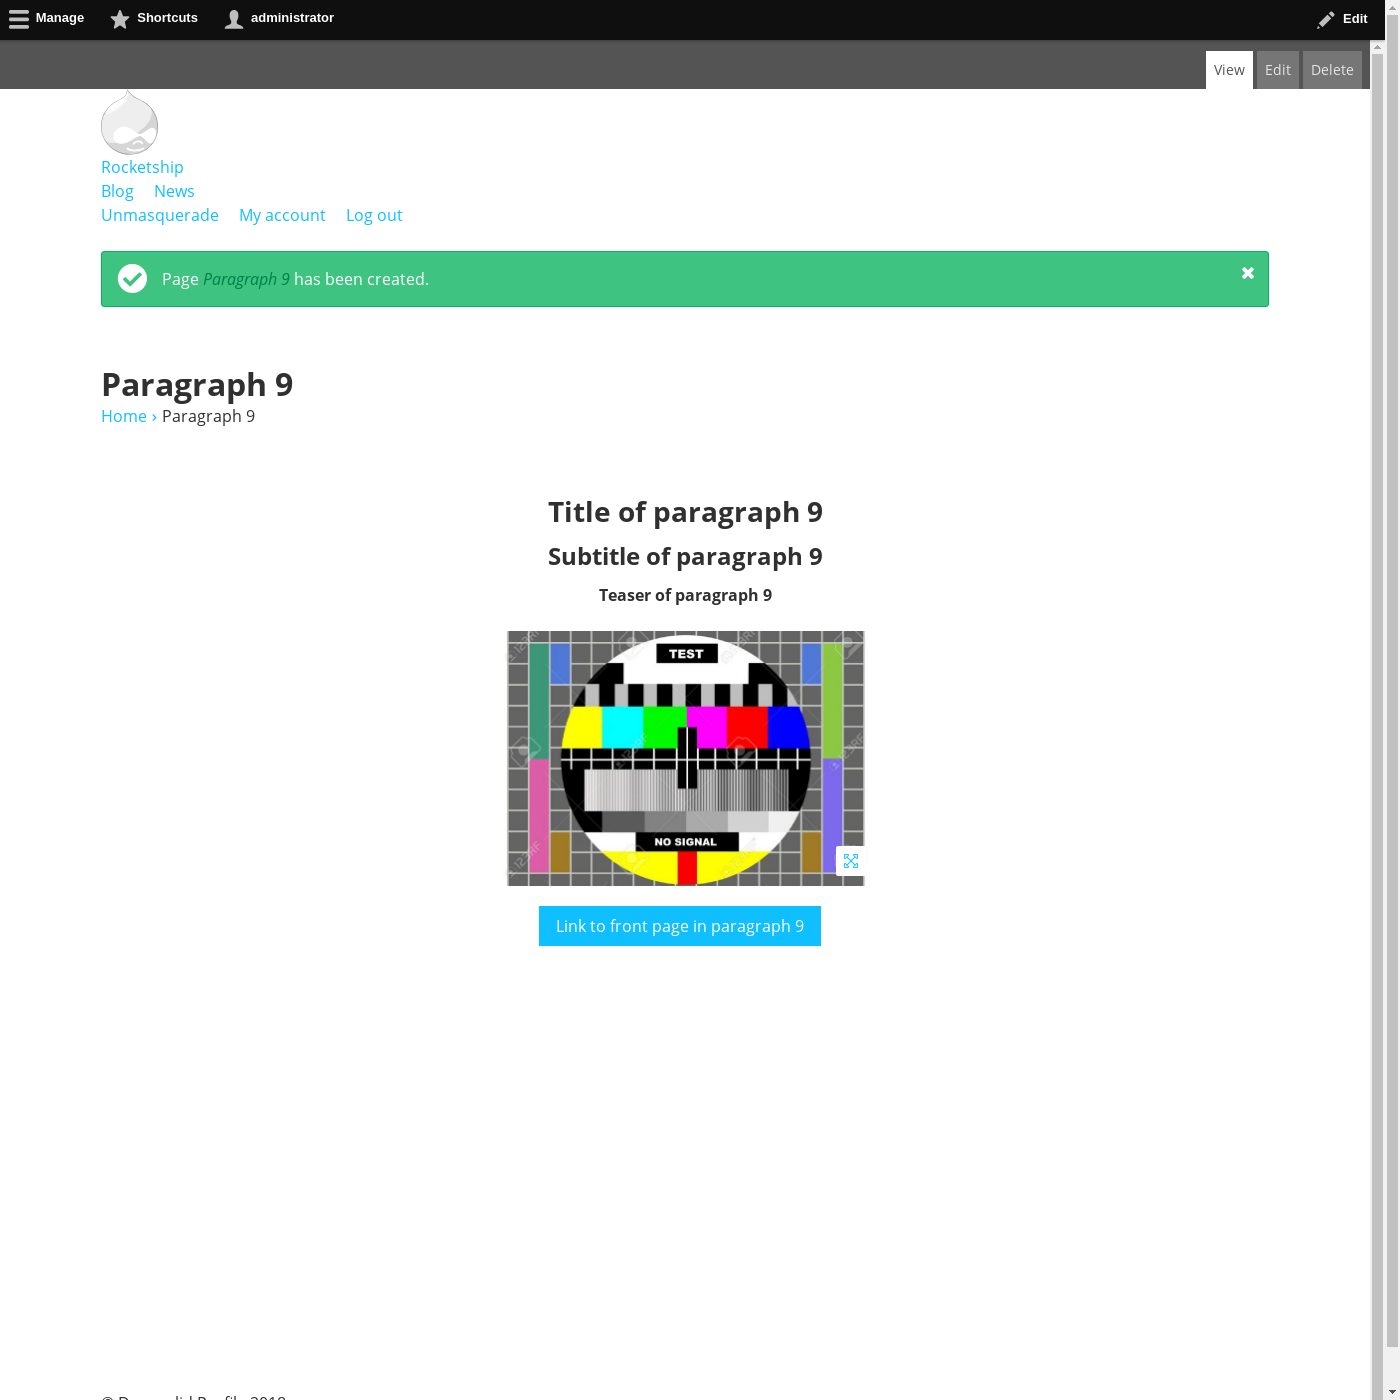
\includegraphics[width=1\textwidth]{img/p009.png}
\end{figure}

\clearpage
\subsection{Paragraph 10: Logo bar}
De tiende Paragraph is een blok met een titel, subtitel, teaser, logo en button met een link.
\begin{figure}[h]
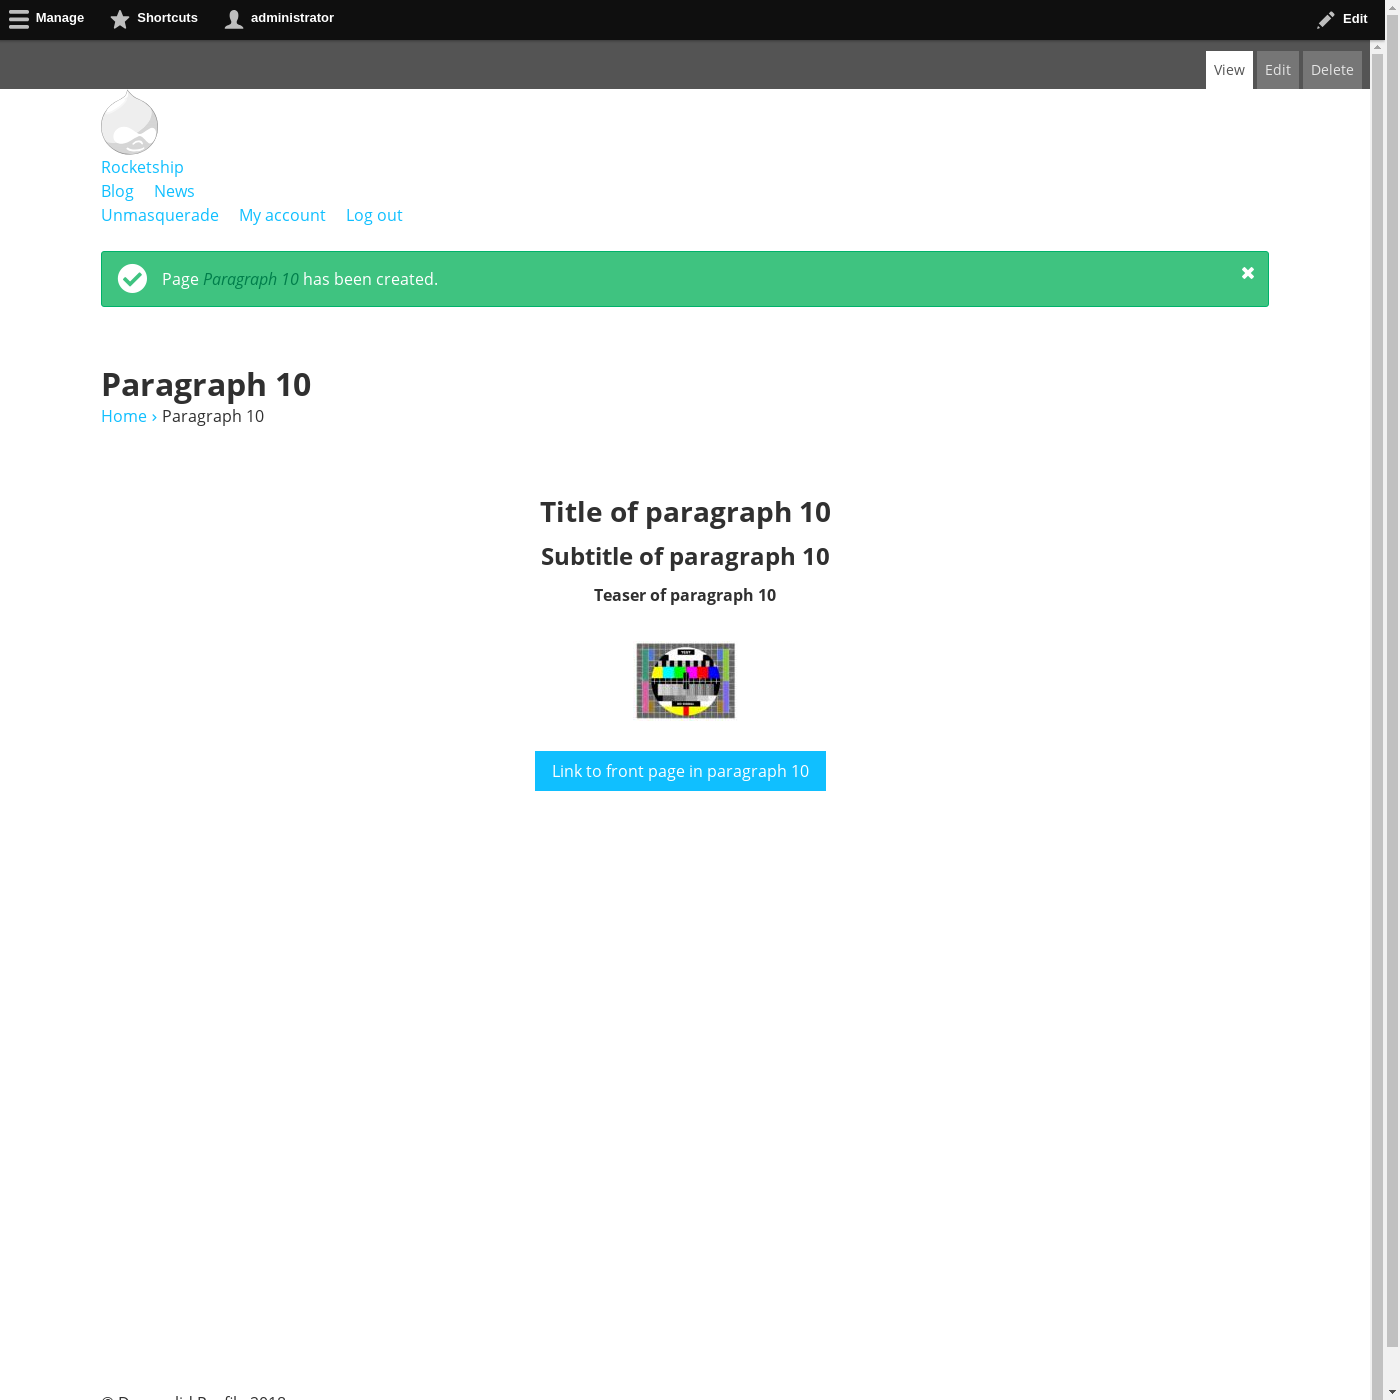
\includegraphics[width=1\textwidth]{img/p010.png}
\end{figure}

\clearpage
\subsection{Paragraph 11: Form}
De elfde Paragraph is een blok met een formulier. Momenteel is het contact formulier het enige formulier dat met deze Paragraph kan aangemaakt worden.
\begin{figure}[h]
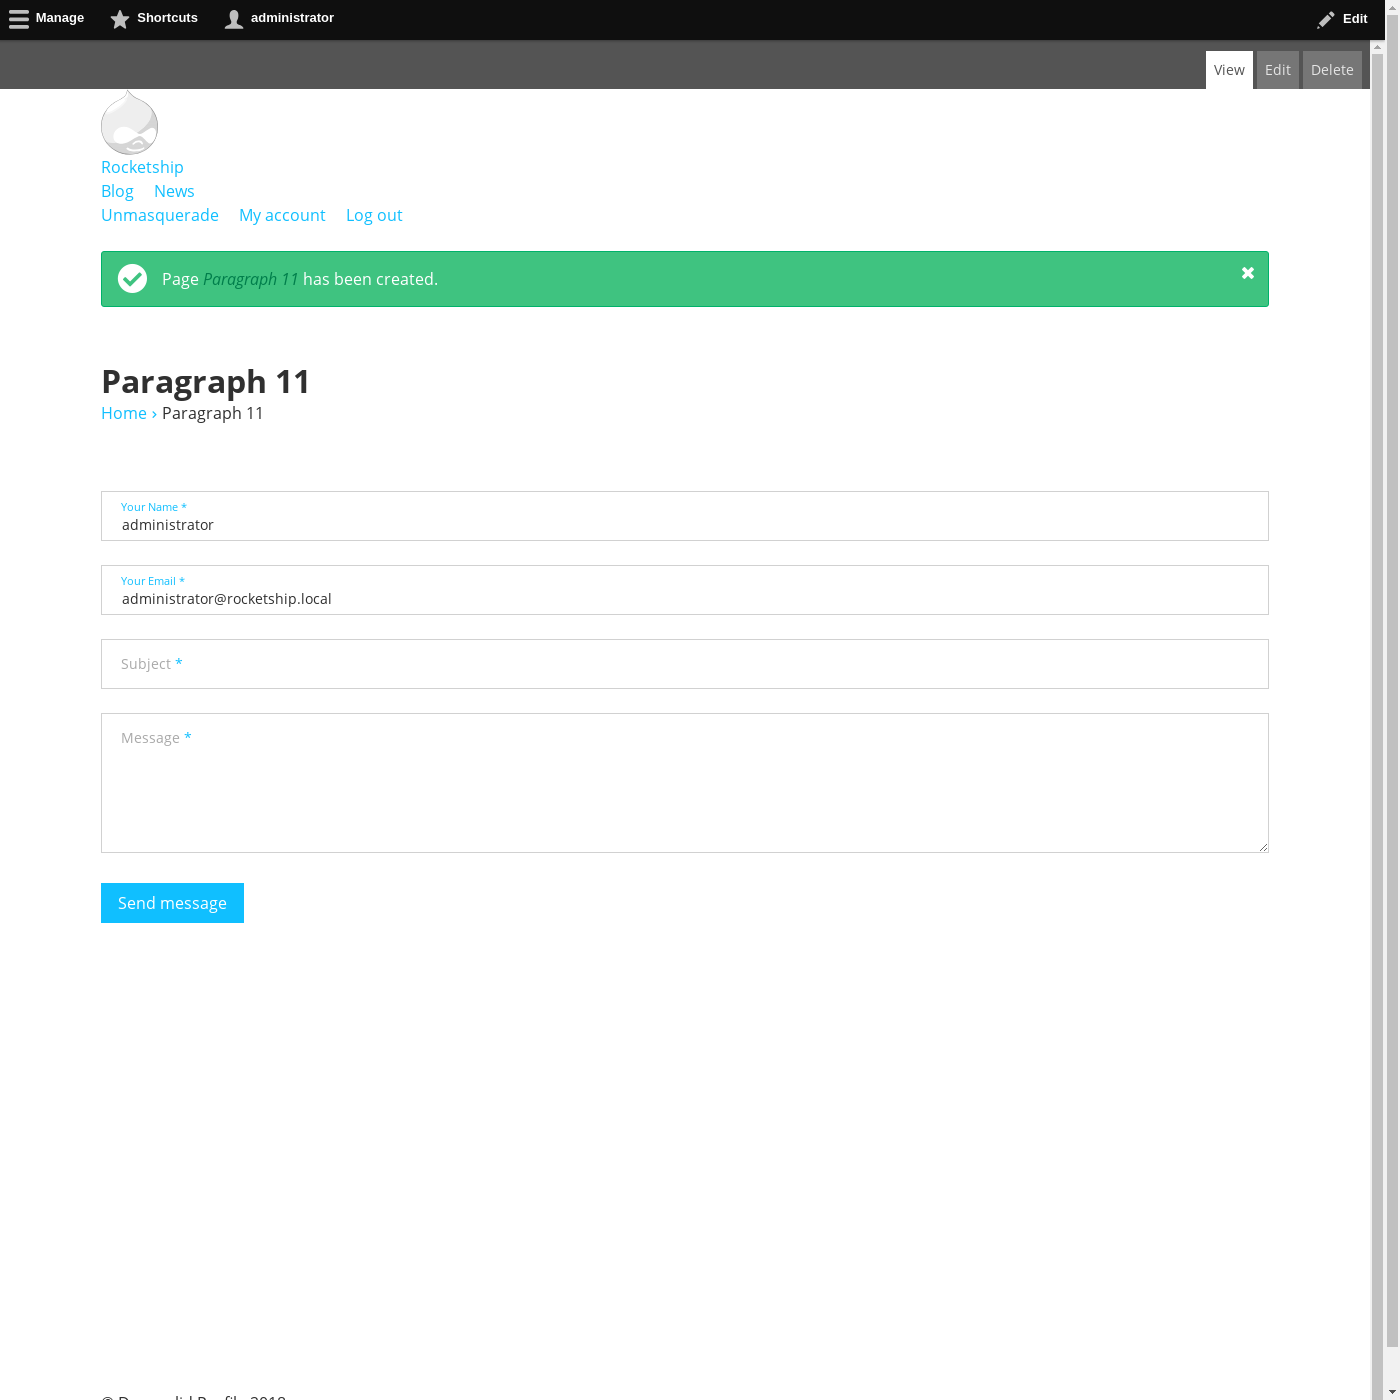
\includegraphics[width=1\textwidth]{img/p011.png}
\end{figure}


\clearpage
\subsection{Paragraph 12: Guidance}
De twaalfde Paragraph is een blok die Guidance items bevat en deze items kunnen op verschillende manieren op de pagina geplaatsts worden, bijvoorbeeld per 2 of per 4 naast elkaar. Zo een Guidance item bevat een titel en een teaser en linkt naar een andere pagina. De blok wordt afgesloten met een button die een link bevat.
\begin{figure}[h]
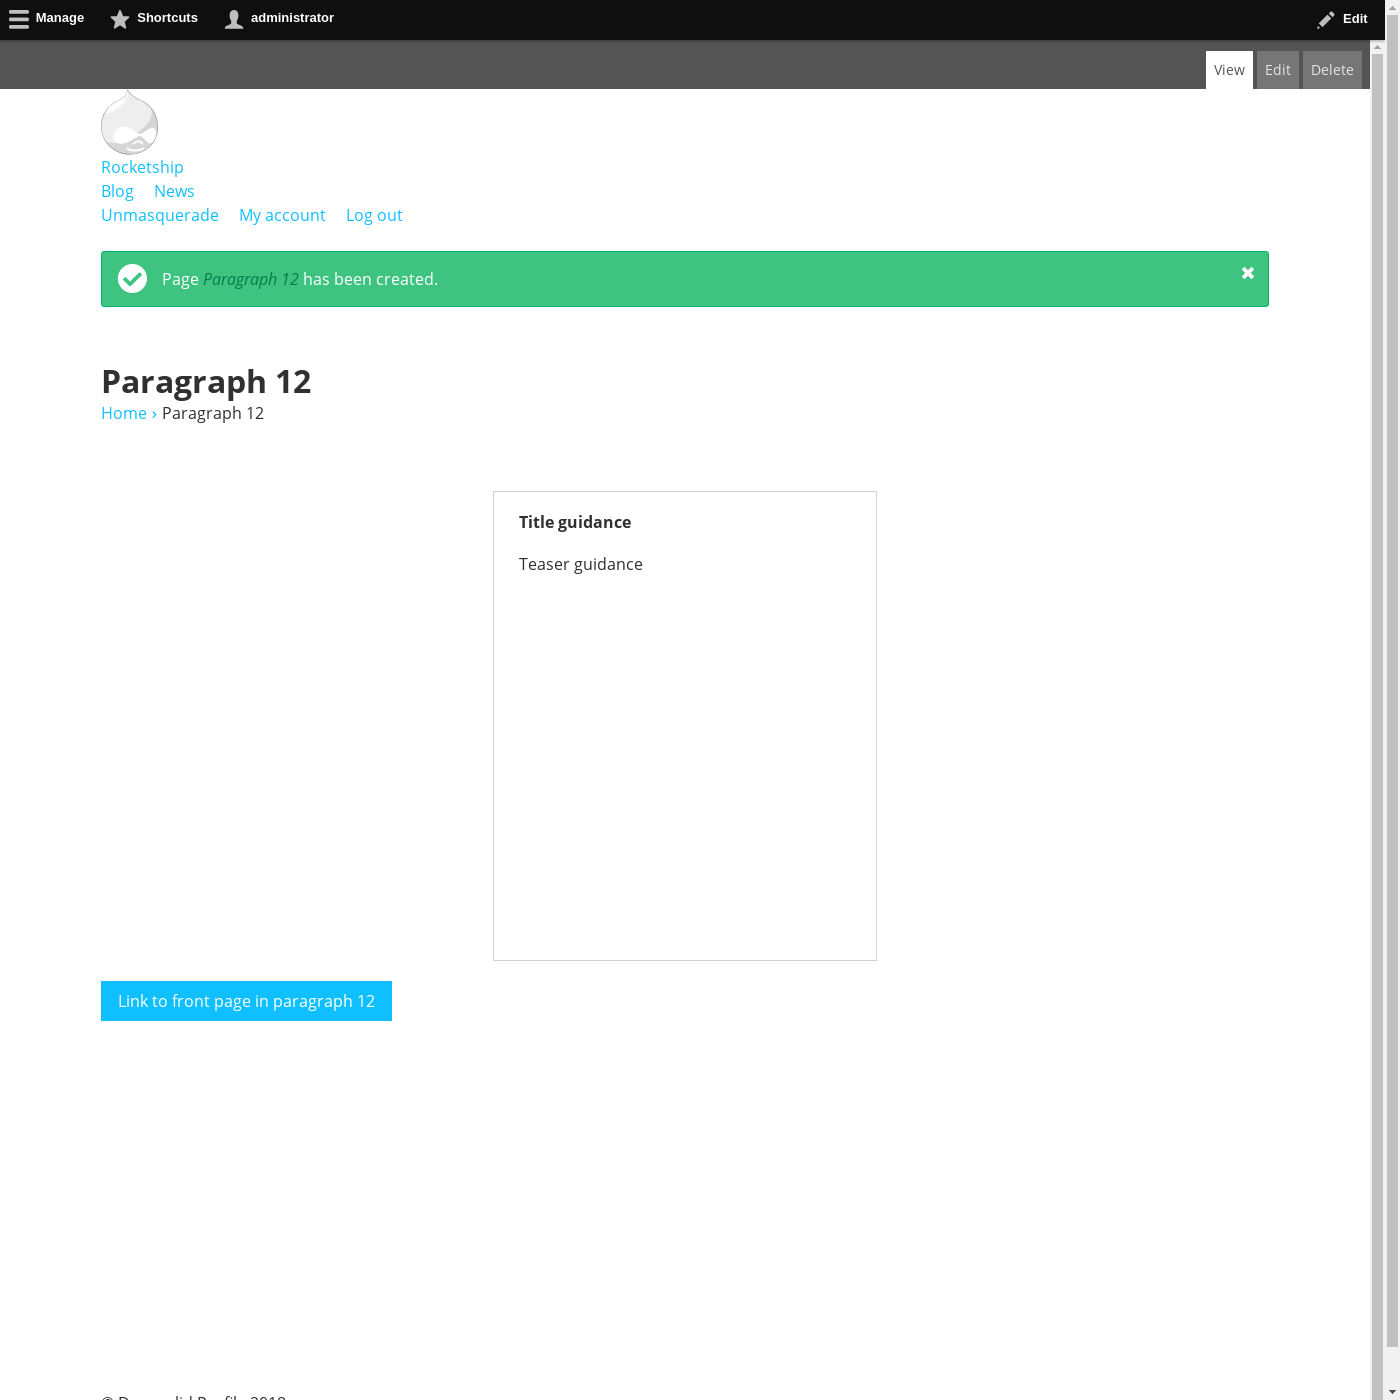
\includegraphics[width=1\textwidth]{img/p012.png}
\end{figure}

\clearpage
\section{Installatie en configuratie}
De installatie begon net zoals in het hoofdstuk methodologie met de lokale en globale installatie van Nightwatch op Rocketship met de respectievelijke commando's "npm install nightwatch", "npm install -g nightwatch".

Voor deze proof of concept wordt gebruik gemaakt van de \textcite{SeleniumStandaloneServer} om de mogelijkheden in verband met het parallel uitvoeren van testen en cross-browser testen aan te tonen. \textcite{ChromeDriver2018} en \textcite{GeckoDriver} worden gedownload met "npm install chromedriver geckodriver". Hiermee kunnen de testen uitgevoerd worden op Google Chrome en op Mozilla Firefox.

Er werden twee configuratiebestanden aangemaakt. Een globals.js bestand dat de globale variabelen bevat en een nightwatch.json bestand dat de hoofdconfiguratie bevat. Hierin staat de configuratie voor het parallel uitvoeren van testen, de configuratie om Selenium Standalone Server, ChromeDriver en GeckoDriver te gebruiken. Hierin staan ook vijf omgevingen gedefinïeerd. De eerste omgeving is de standaard Chrome omgeving. De tweede omgeving is de Chrome desktop omgeving die de testen uitvoert op de Chrome browser met een resolutie van 1366 pixels breed en 768 pixels hoog. De derde omgeving is de Chrome \gls{headless} omgeving. De vierde omgeving is de Firefox desktop omgeving die de testen uitvoert op de Firefox browser met een resolutie van 1366 pixels breed en 768 pixels hoog. De vijfde en laatste omgeving is de Firefox \gls{headless} omgeving.

\paragraph{globals.js}
\lstinputlisting[breaklines=true]{poc/globals.js}
\clearpage
\paragraph{nightwatch.json}
\lstinputlisting[breaklines=true]{poc/nightwatch.json}

\clearpage
\section{Testsuite}
Elke test start met het openen van een browser, te surfen naar de website en in te loggen als administrator. Dan wordt een pagina aangemaakt met de Paragraph die bij de test hoort en worden de velden van de Paragraph ingevuld. Ten slotte wordt elke test afgesloten met het uitloggen en sluiten van de browser.

\paragraph{Lijst van testen}
\begin{enumerate}
\item \hyperref[test1]{Test Paragraph 1}
\item \hyperref[test2]{Test Paragraph 2}
\item \hyperref[test3]{Test Paragraph 3}
\item \hyperref[test4]{Test Paragraph 4}
\item \hyperref[test5]{Test Paragraph 5}
\item \hyperref[test6]{Test Paragraph 6}
\item \hyperref[test7]{Test Paragraph 7}
\item \hyperref[test8]{Test Paragraph 8}
\item \hyperref[test9]{Test Paragraph 9}
\item \hyperref[test10]{Test Paragraph 10}
\item \hyperref[test11]{Test Paragraph 11}
\item \hyperref[test12]{Test Paragraph 12}
\end{enumerate}

\paragraph{Uitvoeringstijd testsuite}
\begin{tabular}{ |c| c| }
\hline
	Google Chrome standaard & 1 minuut 44 seconden \\
\hline
	Google Chrome desktop & 1 minuut 59 seconden \\
\hline
 	Google Chrome headless & 1 minuut 19 seconden \\
\hline
 	Mozilla Firefox desktop & 2 minuten 10 seconden \\
\hline
 	Mozilla Firefox headless & 1 minuut 36 seconden \\
\hline
\end{tabular}


\clearpage
\paragraph{Test Paragraph 1}
\label{test1}
Opbouw test: 
\begin{itemize}
\item test opstarten zoals in het begin van dit deel toegelicht
\item titel en subtitel invullen
\item tekstveld invullen
\item afbeelding met alt tekst toevoegen
\item de viewmode selecteren, in deze test image\_right
\item button met link en link tekst toevoegen
\item pagina opslaan en aanmaken
\item screenshot nemen van de aangemaakte pagina
\item controleren dat de titel en subtitel correct zijn
\item controleren dat het tekstveld correct is
\item controleren dat de alt tekst van de afbeelding correct is
\item controleren dat de correcte view mode is gebruikt
\item controleren dat de button correct is aangemaakt
\item test afsluiten zoals in het begin van dit deel toegelicht
\end{itemize}
\clearpage
\paragraph{testParagraph001.js}
\lstinputlisting[breaklines=true]{poc/testParagraph001.js}

\clearpage
\paragraph{Test Paragraph 2}
\label{test2}
Opbouw test: 
\begin{itemize}
\item test opstarten zoals in het begin van dit deel toegelicht
\item afbeelding met alt tekst toevoegen
\item link toevoegen aan de afbeelding
\item pagina opslaan en aanmaken
\item screenshot nemen van de aangemaakte pagina
\item controleren dat de alt tekst van de afbeelding correct is
\item controleren dat de link op de afbeelding werkt
\item test afsluiten zoals in het begin van dit deel toegelicht
\end{itemize}
\paragraph{testParagraph002.js}
\lstinputlisting[breaklines=true]{poc/testParagraph002.js}

\clearpage
\paragraph{Test Paragraph 3}
\label{test3}
Opbouw test: 
\begin{itemize}
\item test opstarten zoals in het begin van dit deel toegelicht
\item titel en teaser invullen
\item tekstveld invullen
\item de viewmode selecteren, in deze test centered
\item button met link en link tekst toevoegen
\item pagina opslaan en aanmaken
\item screenshot nemen van de aangemaakte pagina
\item controleren dat de titel en teaser correct zijn
\item controleren dat het tekstveld correct is
\item controleren dat de correcte view mode is gebruikt
\item controleren dat de button correct is aangemaakt
\item test afsluiten zoals in het begin van dit deel toegelicht
\end{itemize}
\paragraph{testParagraph003.js}
\lstinputlisting[breaklines=true]{poc/testParagraph003.js}

\clearpage
\paragraph{Test Paragraph 4}
\label{test4}
Opbouw test: 
\begin{itemize}
\item test opstarten zoals in het begin van dit deel toegelicht
\item titel, subtitel en teaser invullen
\item titel  en tekstveld van een FAQ item invullen
\item button met link en link tekst toevoegen
\item pagina opslaan en aanmaken
\item screenshot nemen van de aangemaakte pagina
\item controleren dat de titel, subtitel en teaser correct zijn
\item controleren dat het FAQ item correct is aangemaakt
\item controleren dat de button correct is aangemaakt
\item test afsluiten zoals in het begin van dit deel besproken
\end{itemize}
\paragraph{testParagraph004.js}
\lstinputlisting[breaklines=true]{poc/testParagraph004.js}

\clearpage
\paragraph{Test Paragraph 5}
\label{test5}
Opbouw test: 
\begin{itemize}
\item test opstarten zoals in het begin van dit deel toegelicht
\item afbeelding met alt tekst toevoegen
\item tekstveld invullen
\item Testimonial naam en extra regel invullen
\item Link aan testimonial toevoegen
\item pagina opslaan en aanmaken
\item screenshot nemen van de aangemaakte pagina
\item controleren dat het tekstveld correct is
\item controleren dat de naam en extra regel van het Testimonial item correct zijn
\item controleren dat de alt tekst van de afbeelding correct is
\item controleren dat de correcte view mode is gebruikt
\item controleren dat de Testimonial link correct werkt
\item test afsluiten zoals in het begin van dit deel toegelicht
\end{itemize}
\paragraph{testParagraph005.js}
\lstinputlisting[breaklines=true]{poc/testParagraph005.js}

\clearpage
\paragraph{Test Paragraph 6}
\label{test6}
Opbouw test: 
\begin{itemize}
\item test opstarten zoals in het begin van dit deel toegelicht
\item video link toevoegen
\item pagina opslaan en aanmaken
\item screenshot nemen van de aangemaakte pagina
\item controleren de video is correct is toegevoegd
\item test afsluiten zoals in het begin van dit deel toegelicht
\end{itemize}
\paragraph{testParagraph006.js}
\lstinputlisting[breaklines=true]{poc/testParagraph006.js}

\clearpage
\paragraph{Test Paragraph 7}
\label{test7}
Opbouw test: 
\begin{itemize}
\item test opstarten zoals in het begin van dit deel toegelicht
\item titel, subtitel en teaser invullen
\item titel van het USP item invullen
\item afbeelding met alt tekst toevoegen aan het USP item
\item tekstveld van het USP item invullen
\item link aan het USP item toevoegen
\item button met link en link tekst toevoegen
\item pagina opslaan en aanmaken
\item screenshot nemen van de aangemaakte pagina
\item controleren dat de titel, subtitel en teaser correct zijn
\item controleren dat de titel en tekstveld van het USP item correct zijn
\item controleren dat de alt tekst van de afbeelding van het USP item correct is
\item controleren dat de link van het USP item correct werkt
\item controleren dat de button correct is aangemaakt
\item test afsluiten zoals in het begin van dit deel toegelicht
\end{itemize}
\clearpage
\paragraph{testParagraph007.js}
\lstinputlisting[breaklines=true]{poc/testParagraph007.js}

\clearpage
\paragraph{Test Paragraph 8}
\label{test8}
Opbouw test: 
\begin{itemize}
\item test opstarten zoals in het begin van dit deel toegelicht
\item titel, subtitel en teaser invullen
\item button met link en link tekst toevoegen
\item pagina opslaan en aanmaken
\item screenshot nemen van de aangemaakte pagina
\item controleren dat de titel, subtitel en teaser correct zijn
\item controleren dat de button correct is aangemaakt
\item test afsluiten zoals in het begin van dit deel toegelicht
\end{itemize}
\paragraph{testParagraph008.js}
\lstinputlisting[breaklines=true]{poc/testParagraph008.js}

\clearpage
\paragraph{Test Paragraph 9}
\label{test9}
Opbouw test: 
\begin{itemize}
\item test opstarten zoals in het begin van dit deel toegelicht
\item titel, subtitel en teaser invullen
\item afbeelding met alt tekst toevoegen
\item button met link en link tekst toevoegen
\item pagina opslaan en aanmaken
\item screenshot nemen van de aangemaakte pagina
\item controleren dat de titel, subtitel en teaser correct zijn
\item controleren dat de alt tekst van de afbeelding correct is
\item controleren dat de button correct is aangemaakt
\item test afsluiten zoals in het begin van dit deel toegelicht
\end{itemize}
\paragraph{testParagraph009.js}
\lstinputlisting[breaklines=true]{poc/testParagraph009.js}

\clearpage
\paragraph{Test Paragraph 10}
\label{test10}
Opbouw test: 
\begin{itemize}
\item test opstarten zoals in het begin van dit deel toegelicht
\item titel, subtitel en teaser invullen
\item logo met alt tekst toevoegen
\item link aan het logo toevoegen
\item button met link en link tekst toevoegen
\item pagina opslaan en aanmaken
\item screenshot nemen van de aangemaakte pagina
\item controleren dat de titel, subtitel en teaser correct zijn
\item controleren dat de alt tekst van het logo correct is
\item controleren dat de link van het logo correct werkt
\item controleren dat de button correct is aangemaakt
\item test afsluiten zoals in het begin van dit deel toegelicht
\end{itemize}
\paragraph{testParagraph010.js}
\lstinputlisting[breaklines=true]{poc/testParagraph010.js}

\clearpage
\paragraph{Test Paragraph 11}
\label{test11}
Opbouw test: 
\begin{itemize}
\item test opstarten zoals in het begin van dit deel toegelicht
\item contact formulier selecteren
\item pagina opslaan en aanmaken
\item screenshot nemen van de aangemaakte pagina
\item controleren dat het contact formulier correct is aangemaakt en werkt
\item test afsluiten zoals in het begin van dit deel toegelicht
\end{itemize}
\paragraph{testParagraph011.js}
\lstinputlisting[breaklines=true]{poc/testParagraph011.js}

\clearpage
\paragraph{Test Paragraph 12}
\label{test12}
Opbouw test: 
\begin{itemize}
\item test opstarten zoals in het begin van dit deel toegelicht
\item de viewmode selecteren, hier default\_large
\item titel en teaser van Guidance item invullen
\item afbeelding met alt tekst toevoegen aan het Guidance item
\item link aan het Guidance item toevoegen
\item button met link en link tekst toevoegen
\item pagina opslaan en aanmaken
\item screenshot nemen van de aangemaakte pagina
\item controleren dat de titel en teaser van het Guidance item correct zijn
\item controleren dat de link van het Guidance item correct werkt
\item controleren dat de button correct is aangemaakt
\item test afsluiten zoals in het begin van dit deel toegelicht
\end{itemize}
\paragraph{testParagraph012.js}
\lstinputlisting[breaklines=true]{poc/testParagraph012.js}

\clearpage
\section{Commando's}
Voor de testen zo leesbaar en gebruiksvriendelijk mogelijk te maken werden er commando's geschreven die de achterliggende code weg abstraheren.

\paragraph{Lijst van commando's}
\begin{enumerate}
\item \hyperref[commando1]{drupalAssertParagraphButton}
\item \hyperref[commando2]{drupalAssertParagraphCkeditor}
\item \hyperref[commando3]{drupalAssertParagraphFaq}
\item \hyperref[commando4]{drupalAssertParagraphForm}
\item \hyperref[commando5]{drupalAssertParagraphGuidance}
\item \hyperref[commando6]{drupalAssertParagraphImage}
\item \hyperref[commando7]{drupalAssertParagraphLink}
\item \hyperref[commando8]{drupalAssertParagraphTestimonial}
\item \hyperref[commando9]{drupalAssertParagraphTitle}
\item \hyperref[commando10]{drupalAssertParagraphUsp}
\item \hyperref[commando11]{drupalAssertParagraphVideo}
\item \hyperref[commando12]{drupalAssertParagraphViewmode}
\item \hyperref[commando13]{drupalCreatePageWithParagraph}
\item \hyperref[commando14]{drupalDeletePage}
\item \hyperref[commando15]{drupalInputParagraphButton}
\item \hyperref[commando16]{drupalInputParagraphCkeditor}
\item \hyperref[commando17]{drupalInputParagraphFaq}
\item \hyperref[commando18]{drupalInputParagraphForm}
\item \hyperref[commando19]{drupalInputParagraphGuidance}
\item \hyperref[commando20]{drupalInputParagraphImage}
\item \hyperref[commando21]{drupalInputParagraphLink}
\item \hyperref[commando22]{drupalInputParagraphTestimonial}
\item \hyperref[commando23]{drupalInputParagraphTitle}
\item \hyperref[commando24]{drupalInputParagraphUsp}
\item \hyperref[commando25]{drupalInputParagraphVideo}
\item \hyperref[commando26]{drupalInputParagraphViewmode}
\item \hyperref[commando27]{drupalLogin}
\item \hyperref[commando28]{drupalLoginAsAdmin}
\item \hyperref[commando29]{drupalLogout}
\item \hyperref[commando30]{drupalRelativeURL}
\item \hyperref[commando31]{drupalScreenshot}
\item \hyperref[commando32]{drupalSubmit}
\item \hyperref[commando33]{drupalUserIsLoggedIn}
\end{enumerate}

\clearpage
\paragraph{drupalAssertParagraphButton}
\label{commando1}
Dit commando gaat na of een button op een Paragraph correct is aangemaakt door de titel te vergelijken met de waarde meegegeven en door op de button te klikken en de url van de bezochte pagina te vergelijken met de meegegeven waarde.
\paragraph{drupalAssertParagraphButton.js}
\begin{lstlisting}[breaklines=true]
exports.command = function drupalAssertParagraphButton({ title, url }) {
  if (typeof title !== 'undefined') {
    this.assert.containsText('.paragraph .field--name-field-p-button a', title);
  }

  if (typeof url !== 'undefined') {
    this.waitForElementVisible('.paragraph .field--name-field-p-button a', this.globals.timeoutTime)
      .click('.paragraph .field--name-field-p-button a')
      .assert.urlEquals(url)
      .back();
  }

  return this;
};
\end{lstlisting}


\clearpage
\paragraph{drupalAssertParagraphCkeditor}
\label{commando2}
Dit commando gaat na of het tekstveld op een Paragraph correct is aangemaakt door het te vergelijken met de meegegeven waarde.
\paragraph{drupalAssertParagraphCkeditor.js}
\begin{lstlisting}[breaklines=true]
exports.command = function drupalAssertParagraphCkeditor({ text }) {
  if (typeof text !== 'undefined') {
    this.assert.containsText('.paragraph .field--name-field-p-text p', text);
  }

  return this;
};
\end{lstlisting}


\clearpage
\paragraph{drupalAssertParagraphFaq}
\label{commando3}
Dit commando gaat na of de FAQ Paragraph correct is aangemaakt door de titel en het tekstveld te vergelijken met de meegegeven waarden.
\paragraph{drupalAssertParagraphFaq.js}
\begin{lstlisting}[breaklines=true]
exports.command = function drupalAssertParagraphFaq({ title, ckeditor }) {
  if (typeof title !== 'undefined') {
    this.assert.containsText('.paragraph--type-p-004 .field__item--name-field-p-004-item:first-of-type h3', title);
  }

  if (typeof ckeditor !== 'undefined') {
    this.waitForElementVisible('.paragraph--type-p-004 .field__item--name-field-p-004-item:first-of-type h3', this.globals.timeoutTime)
      .click('.paragraph--type-p-004 .field__item--name-field-p-004-item:first-of-type h3')
      .assert.containsText('.paragraph--type-p-004 .field__item--name-field-p-004-item:first-of-type .tab-item__content', ckeditor);
  }

  return this;
};
\end{lstlisting}


\clearpage
\paragraph{drupalAssertParagraphForm}
\label{commando4}
Dit commando gaat na of de Paragraph met een contact formulier correct is aangemaakt.
\paragraph{drupalAssertParagraphForm.js}
\begin{lstlisting}[breaklines=true]
exports.command = function drupalAssertParagraphForm({ subject, message }) {
  this.waitForElementVisible('input[name="name"]', this.globals.timeoutTime)
    .assert.attributeEquals('input[name="name"]', 'value', this.globals.adminUsername)
    .assert.attributeEquals('input[name="email"]', 'value', this.globals.adminUsername + '@rocketship.local');

  if (typeof subject !== 'undefined') {
    this.setValue('input[name="subject"]', subject);
  }

  if (typeof message !== 'undefined') {
    this.setValue('textarea[name="message"]', message);
  }

  if (typeof subject !== 'undefined' && typeof message !== 'undefined') {
    this.click('#edit-actions-submit')
      .assert.urlEquals(this.globals.launch_url + '/')
      .back();
  }
  return this;
};
\end{lstlisting}


\clearpage
\paragraph{drupalAssertParagraphGuidance}
\label{commando5}
Dit commando gaat na of de Paragraph Guidance titel en teaser correct zijn aangemaakt door deze te vergelijken met de meegegeven waarden.
\paragraph{drupalAssertParagraphGuidance.js}
\begin{lstlisting}[breaklines=true]
exports.command = function drupalAssertParagraphGuidance({ title, teaser }) {
  if (typeof title !== 'undefined') {
    this.assert.containsText('.paragraph--type-p-012 .paragraph--type-p-012-child .field--name-field-p-title h4', title);
  }

  if (typeof teaser !== 'undefined') {
    this.assert.containsText('.paragraph--type-p-012 .paragraph--type-p-012-child .field--name-field-p-teaser', teaser);
  }

  return this;
};
\end{lstlisting}


\clearpage
\paragraph{drupalAssertParagraphImage}
\label{commando6}
Dit commando gaat na of een Paragraph afbeelding correct is aangemaakt door de alt tag te vergelijken met de meegegeven waarde. Voor de afbeeldingen van Paragraph 7 en 9 moet een ander argument meegegeven worden.
\paragraph{drupalAssertParagraphImage.js}
\begin{lstlisting}[breaklines=true]
exports.command = function drupalAssertParagraphImage({ alt, altp007, altp009 }) {
  if (typeof alt !== 'undefined') {
    this.assert.attributeEquals('.paragraph .field--name-field-p-image img', 'alt', alt);
  }

  if (typeof altp007 !== 'undefined') {
    this.assert.attributeEquals('.paragraph--type-p-007 .field__item--name-field-p-007-children .field--name-image-url-field img', 'alt', altp007);
  }

  if (typeof altp009 !== 'undefined') {
    this.assert.attributeEquals('.paragraph--type-p-009 .field--name-field-p-images-unlimited img', 'alt', altp009);
  }

  return this;
};
\end{lstlisting}


\clearpage
\paragraph{drupalAssertParagraphLink}
\label{commando7}
Dit commando gaat na of de Paragraph link correct is aangemaakt door de titel er van te vergelijken met de meegegeven waarde en door op de link te klikken en de url te vergelijken met de meegegeven waarde. Voor Paragraph 7 moet een andere url argument meegegeven worden.
\paragraph{drupalAssertParagraphLink.js}
\begin{lstlisting}[breaklines=true]
exports.command = function drupalAssertParagraphLink({ title, url, urlp007 }) {
  if (typeof title !== 'undefined') {
    this.assert.containsText('.paragraph .field--name-field-p-link  a', title);
  }

  if (typeof url !== 'undefined') {
    this.waitForElementVisible('.paragraph .field--name-field-p-link  a', this.globals.timeoutTime)
      .click('.paragraph .field--name-field-p-link  a')
      .assert.urlEquals(url)
      .back();
  }

  if (typeof urlp007 !== 'undefined') {
    this.waitForElementVisible('.paragraph--type-p-007 .field__item--name-field-p-007-children .field--name-image-url-field a', this.globals.timeoutTime)
      .click('.paragraph--type-p-007 .field__item--name-field-p-007-children .field--name-image-url-field a')
      .assert.urlEquals(urlp007)
      .back();
  }

  return this;
};
\end{lstlisting}


\clearpage
\paragraph{drupalAssertParagraphTestimonial}
\label{commando8}
Dit commando gaat na of de Paragraph Testimonial correct is aangemaakt door de naam en extra regel te vergelijken met de meegegeven waarden.
\paragraph{drupalAssertParagraphTestimonial.js}
\begin{lstlisting}[breaklines=true]
exports.command = function drupalAssertParagraphTestimonial({name, extrarule}) {
  if(typeof name !== 'undefined') {
    this.assert.containsText('.paragraph--type-p-005 .field--name-field-p-name', name);
  }

  if(typeof extrarule !== 'undefined') {
    this.assert.containsText('.paragraph--type-p-005 .field--name-field-p-extra-rule', extrarule);
  }
  
  return this;
};
\end{lstlisting}


\clearpage
\paragraph{drupalAssertParagraphTitle}
\label{commando9}
Dit commando gaat na of de Paragraph titel, subtitel of teaser correct zijn aangemaakt door deze te vergelijken met de meegegeven waarden.
\paragraph{drupalAssertParagraphTitle.js}
\begin{lstlisting}[breaklines=true]
exports.command = function drupalAssertParagraphTitle({ title, subtitle, teaser }) {
  if (typeof title !== 'undefined') {
    this.assert.containsText('.paragraph .field--name-field-p-title h2', title);
  }

  if (typeof subtitle !== 'undefined') {
    this.assert.containsText('.paragraph .field--name-field-p-subtitle h3', subtitle);
  }

  if (typeof teaser !== 'undefined') {
    this.assert.containsText('.paragraph .field--name-field-p-teaser', teaser);
  }
  
  return this;
};
\end{lstlisting}


\clearpage
\paragraph{drupalAssertParagraphUsp}
\label{commando10}
Dit commando gaat na of de Paragraph USP correct is aangemaakt door de titel en tekst er van te vergelijken met de meegegeven waarden.
\paragraph{drupalAssertParagraphUsp.js}
\begin{lstlisting}[breaklines=true]
exports.command = function drupalAssertParagraphUsp({ title, text }) {
  if (typeof title !== 'undefined') {
    this.assert.containsText('.paragraph--type-p-007 .field__item--name-field-p-007-children .field--name-field-p-title h3', title);
  }

  if (typeof text !== 'undefined') {
    this.assert.containsText('.paragraph--type-p-007 .field__item--name-field-p-007-children .field--name-field-p-text p', text);
  }

  return this;
};
\end{lstlisting}


\clearpage
\paragraph{drupalAssertParagraphVideo}
\label{commando11}
Dit commando gaat na of de Paragraph video is aangemaakt en een video bevat.
\paragraph{drupalAssertParagraphVideo.js}
\begin{lstlisting}[breaklines=true]
exports.command = function drupalAssertParagraphVideo() {
  this.waitForElementVisible('.paragraph--type-p-006 .field--type-video-embed-field iframe', this.globals.timeoutTime);

  return this;
};
\end{lstlisting}


\clearpage
\paragraph{drupalAssertParagraphViewmode}
\label{commando12}
Dit commando gaat na of de juiste Paragraph viewmode is gebruikt. De argumenten die kunnen meegegeven worden zijn specifiek voor Paragraph 1 of Paragraph 3.
\paragraph{drupalAssertParagraphViewmode.js}
\begin{lstlisting}[breaklines=true]
exports.command = function drupalAssertParagraphViewmode({ viewmodep001, viewmodep003 }) {
  if (typeof viewmodep001 !== 'undefined') {
    switch (viewmodep001) {
      case 'image_right':
        this.assert.cssProperty('.paragraph .field--image', 'float', 'right');
        break;
      case 'image_left':
        this.assert.cssProperty('.paragraph .field--image', 'float', 'left');
        break;
    }
  }

  if (typeof viewmodep003 !== 'undefined') {
    switch (viewmodep003) {
      case 'centered':
        this.assert.cssProperty('.p-003--view-mode--centered', 'text-align', 'center');
        break;
      case 'left':
        this.assert.cssProperty('.p-003--view-mode--left', 'text-align', 'left');
        break;
    }
  }

  return this;
};
\end{lstlisting}


\clearpage
\paragraph{drupalCreatePageWithParagraph}
\label{commando13}
Dit commando maakt een pagina aan met de titel en beschrijving die meegegeven worden en selecteert de Paragraph die hoort bij de waarde die meegegeven is.
\paragraph{drupalCreatePageWithParagraph.js}
\begin{lstlisting}[breaklines=true]
exports.command = function drupalCreatePageWithParagraph({ pageTitle, pageDescription, paragraphValue }) {
  if (typeof pageTitle !== 'undefined') {
    this.drupalRelativeURL('/node/add/page')
      .waitForElementVisible('input[id=edit-title-0-value]', this.globals.timeoutTime)
      .setValue('input[id=edit-title-0-value]', pageTitle);
  }

  if (typeof pageDescription !== 'undefined') {
    this.waitForElementVisible('#edit-field-description-0-value', this.globals.timeoutTime)
      .setValue('#edit-field-description-0-value', pageDescription);
  }

  if (typeof paragraphValue !== 'undefined') {
    this.waitForElementVisible('#edit-field-paragraphs-add-more-add-more-select option[value=' + paragraphValue + ']', this.globals.timeoutTime)
      .click('#edit-field-paragraphs-add-more-add-more-select option[value=' + paragraphValue + ']')
      .click('#edit-field-paragraphs-add-more-add-more-button')
      .waitForElementVisible('input[value="Add another Paragraph"]', this.globals.timeoutTime);
  }

  return this;
};
\end{lstlisting}


\clearpage
\paragraph{drupalDeletePage}
\label{commando14}
Dit commando verwijdert de pagina waarop de gebruiker aanwezig is.
\paragraph{drupalDeletePage.js}
\begin{lstlisting}[breaklines=true]
exports.command = function drupalDeletePage() {
  this.waitForElementPresent('#block-dropsolid-starter-local-tasks', this.globals.timeoutTime)
    .execute(function () {
      document.querySelector('#block-dropsolid-starter-local-tasks .tabs__nav--local-tasks li:last-child a').click();
    })
    .drupalSubmit();

  return this;
};
\end{lstlisting}


\clearpage
\paragraph{drupalInputParagraphButton}
\label{commando15}
Dit commando voert de waarden voor het aanmaken van een Paragraph button in met de waarden die zijn meegegeven. Dit zijn de titel van de button, de link van de button en de target (open de pagina in hetzelfde of in een ander tabblad).
\paragraph{drupalInputParagraphButton.js}
\begin{lstlisting}[breaklines=true]
exports.command = function drupalInputParagraphButton({ url, title, target }) {
  if (typeof url !== 'undefined') {
    this.waitForElementVisible('input[name="field_paragraphs[0][subform][field_p_button][0][uri]"]', this.globals.timeoutTime)
      .setValue('input[name="field_paragraphs[0][subform][field_p_button][0][uri]"]', url);
  }

  if (typeof title !== 'undefined') {
    this.waitForElementVisible('input[name="field_paragraphs[0][subform][field_p_button][0][title]"]', this.globals.timeoutTime)
      .setValue('input[name="field_paragraphs[0][subform][field_p_button][0][title]"]', title);
  }

  if (typeof target !== 'undefined') {
    this.waitForElementVisible('select[name="field_paragraphs[0][subform][field_p_button][0][options][attributes][target]"] option[value= ' + target + ']', this.globals.timeoutTime)
      .click('select[name="field_paragraphs[0][subform][field_p_button][0][options][attributes][target]"] option[value= ' + target + ']');
  }

  return this;
};
\end{lstlisting}


\clearpage
\paragraph{drupalInputParagraphCkeditor}
\label{commando16}
Dit commando voert de waarde van een Paragraph tekstveld in met de waarde die is meegegeven.
\paragraph{drupalInputParagraphCkeditor.js}
\begin{lstlisting}[breaklines=true]
exports.command = function drupalInputParagraphCkeditor({ text }) {
  if (typeof text !== 'undefined') {
    var ckeditor;
    this.execute(
      function (instance, content) {
        for (var i in CKEDITOR.instances)
          CKEDITOR.instances[i].setData(content);
      },
      [
        ckeditor,
        text
      ]
    );
  }

  return this;
};
\end{lstlisting}


\clearpage
\paragraph{drupalInputParagraphFaq}
\label{commando17}
Dit commando voert de tekst van de Paragraph FAQ in met de waarde die is meegegeven.
\paragraph{drupalInputParagraphFaq.js}
\begin{lstlisting}[breaklines=true]
exports.command = function drupalInputParagraphFaq({ text }) {
  if (typeof text !== 'undefined') {
    this.waitForElementVisible('.field--name-field-p-004-item tbody tr:first-child summary[role="button"]', this.globals.timeoutTime)
      .click('.field--name-field-p-004-item tbody tr:first-child summary[role="button"]')
      .setValue('input[name="field_paragraphs[0][subform][field_p_004_item][0][container_1][title]"]', text);
  }

  return this;
};
\end{lstlisting}


\clearpage
\paragraph{drupalInputParagraphForm}
\label{commando18}
Dit commando selecteert de waarde van de form die in Paragraph form kan aangemaakt worden met de waarde die is meegegeven.
\paragraph{drupalInputParagraphForm.js}
\begin{lstlisting}[breaklines=true]
exports.command = function drupalInputParagraphForm({ form }) {
  if (typeof form !== 'undefined') {
    this.waitForElementVisible('select[name="field_paragraphs[0][subform][field_webform][0][target_id]"]', this.globals.timeoutTime)
      .click('select[name="field_paragraphs[0][subform][field_webform][0][target_id]"] option[value=' + form + ']');
  }

  return this;
};
\end{lstlisting}


\clearpage
\paragraph{drupalInputParagraphGuidance}
\label{commando19}
Dit commando vult de titel en teaser van Paragraph Guidance in met de meegegeven waarden.
\paragraph{drupalInputParagraphGuidance.js}
\begin{lstlisting}[breaklines=true]
exports.command = function drupalInputParagraphGuidance({ title, teaser }) {
  this.waitForElementVisible('summary[role="button"]', this.globals.timeoutTime)
    .click('summary[role="button"]');

  if (typeof title !== 'undefined') {
    this.setValue('input[name="field_paragraphs[0][subform][field_p_012_children][0][subform][field_p_title][0][value]"]', title);
  }

  if (typeof teaser !== 'undefined') {
    this.setValue('textarea[name="field_paragraphs[0][subform][field_p_012_children][0][subform][field_p_teaser][0][value]"]', teaser);
  }

  return this;
};
\end{lstlisting}


\clearpage
\paragraph{drupalInputParagraphImage}
\label{commando20}
Dit commando voegt een afbeelding toe aan een Paragraph door de afbeelding en alt tekst in te vullen met de meegegeven waarden. Voor Paragraph 7, 9, 10 en 12 moeten andere argumenten gebruikt worden.
\paragraph{drupalInputParagraphImage.js}
\begin{lstlisting}[breaklines=true]
exports.command = function drupalInputParagraphImage({ image, alt, imagep007, altp007, imagep009, altp009, imagep010, altp010, imagep012, altp012 }) {
  if (typeof image !== 'undefined') {
    this.waitForElementVisible('input[name="files[field_paragraphs_0_subform_field_p_image_0]"]', this.globals.timeoutTime)
      .setValue('input[name="files[field_paragraphs_0_subform_field_p_image_0]"]', require('path').resolve(__dirname + '/images/' + image));
  }

  if (typeof alt !== 'undefined') {
    this.waitForElementVisible('input[name="field_paragraphs[0][subform][field_p_image][0][alt]"]', this.globals.timeoutTime)
      .setValue('input[name="field_paragraphs[0][subform][field_p_image][0][alt]"]', alt);
  }

  if (typeof imagep007 !== 'undefined') {
    this.waitForElementVisible('input[name="files[field_paragraphs_0_subform_field_p_007_children_0_subform_field_p_image_0]"]', this.globals.timeoutTime)
      .setValue('input[name="files[field_paragraphs_0_subform_field_p_007_children_0_subform_field_p_image_0]"]', require('path').resolve(__dirname + '/images/' + imagep007));
  }

  if (typeof altp007 !== 'undefined') {
    this.waitForElementVisible('input[name="field_paragraphs[0][subform][field_p_007_children][0][subform][field_p_image][0][alt]"]', this.globals.timeoutTime)
      .setValue('input[name="field_paragraphs[0][subform][field_p_007_children][0][subform][field_p_image][0][alt]"]', altp007);
  }

  if (typeof imagep009 !== 'undefined') {
    this.waitForElementVisible('input[name="files[field_paragraphs_0_subform_field_p_images_unlimited_0][]"]', this.globals.timeoutTime)
      .setValue('input[name="files[field_paragraphs_0_subform_field_p_images_unlimited_0][]"]', require('path').resolve(__dirname + '/images/' + imagep009));
  }

  if (typeof altp009 !== 'undefined') {
    this.waitForElementVisible('input[name="field_paragraphs[0][subform][field_p_images_unlimited][0][alt]"]', this.globals.timeoutTime)
      .setValue('input[name="field_paragraphs[0][subform][field_p_images_unlimited][0][alt]"]', altp009);
  }

  if (typeof imagep010 !== 'undefined') {
    this.waitForElementVisible('input[name="files[field_paragraphs_0_subform_field_p_010_children_0_subform_field_p_image_0]"]', this.globals.timeoutTime)
      .setValue('input[name="files[field_paragraphs_0_subform_field_p_010_children_0_subform_field_p_image_0]"]', require('path').resolve(__dirname + '/images/' + imagep010));
  }

  if (typeof altp010 !== 'undefined') {
    this.waitForElementVisible('input[name="field_paragraphs[0][subform][field_p_010_children][0][subform][field_p_image][0][alt]"]', this.globals.timeoutTime)
      .setValue('input[name="field_paragraphs[0][subform][field_p_010_children][0][subform][field_p_image][0][alt]"]', altp010);
  }

  if (typeof imagep012 !== 'undefined') {
    this.waitForElementVisible('input[name="files[field_paragraphs_0_subform_field_p_012_children_0_subform_field_p_image_0]"]', this.globals.timeoutTime)
      .setValue('input[name="files[field_paragraphs_0_subform_field_p_012_children_0_subform_field_p_image_0]"]', require('path').resolve(__dirname + '/images/' + imagep012));
  }

  if (typeof altp012 !== 'undefined') {
    this.waitForElementVisible('input[name="field_paragraphs[0][subform][field_p_012_children][0][subform][field_p_image][0][alt]"]', this.globals.timeoutTime)
      .setValue('input[name="field_paragraphs[0][subform][field_p_012_children][0][subform][field_p_image][0][alt]"]', altp012);
  }
  
  return this;
};
\end{lstlisting}


\clearpage
\paragraph{drupalInputParagraphLink}
\label{commando21}
Dit commando vult de url, titel en target (open link in nieuw tabblad of niet) van een link in met de meegegeven waarden.
\paragraph{drupalInputParagraphLink.js}
\begin{lstlisting}[breaklines=true]
exports.command = function drupalInputParagraphLink({ url, title, target, urlp007, titlep007, targetp007, urlp010, titlep010, targetp010, urlp012, titlep012, targetp012 }) {
  if (typeof url !== 'undefined') {
    this.waitForElementVisible('input[name="field_paragraphs[0][subform][field_p_link][0][uri]"]', this.globals.timeoutTime)
      .setValue('input[name="field_paragraphs[0][subform][field_p_link][0][uri]"]', url);
  }

  if (typeof title !== 'undefined') {
    this.waitForElementVisible('input[name="field_paragraphs[0][subform][field_p_link][0][title]"]', this.globals.timeoutTime)
      .setValue('input[name="field_paragraphs[0][subform][field_p_link][0][title]"]', title);
  }

  if (typeof target !== 'undefined') {
    this.waitForElementVisible('select[name="field_paragraphs[0][subform][field_p_link][0][options][attributes][target]"] option[value= ' + target + ']', this.globals.timeoutTime)
      .click('select[name="field_paragraphs[0][subform][field_p_link][0][options][attributes][target]"] option[value= ' + target + ']');
  }

  if (typeof urlp007 !== 'undefined') {
    this.waitForElementVisible('input[name="field_paragraphs[0][subform][field_p_007_children][0][subform][field_p_link][0][uri]"]', this.globals.timeoutTime)
      .setValue('input[name="field_paragraphs[0][subform][field_p_007_children][0][subform][field_p_link][0][uri]"]', urlp007);
  }

  if (typeof titlep007 !== 'undefined') {
    this.waitForElementVisible('input[name="field_paragraphs[0][subform][field_p_007_children][0][subform][field_p_link][0][title]"]', this.globals.timeoutTime)
      .setValue('input[name="field_paragraphs[0][subform][field_p_007_children][0][subform][field_p_link][0][title]"]', titlep007);
  }

  if (typeof targetp007 !== 'undefined') {
    this.waitForElementVisible('select[name="field_paragraphs[0][subform][field_p_007_children][0][subform][field_p_link][0][options][attributes][target]"] option[value= ' + targetp007 + ']', this.globals.timeoutTime)
      .click('select[name="field_paragraphs[0][subform][field_p_007_children][0][subform][field_p_link][0][options][attributes][target]"] option[value= ' + targetp007 + ']');
  }

  if (typeof urlp010 !== 'undefined') {
    this.waitForElementVisible('input[name="field_paragraphs[0][subform][field_p_010_children][0][subform][field_p_link][0][uri]"]', this.globals.timeoutTime)
      .setValue('input[name="field_paragraphs[0][subform][field_p_010_children][0][subform][field_p_link][0][uri]"]', urlp010);
  }

  if (typeof titlep010 !== 'undefined') {
    this.waitForElementVisible('input[name="field_paragraphs[0][subform][field_p_010_children][0][subform][field_p_link][0][title]"]', this.globals.timeoutTime)
      .setValue('input[name="field_paragraphs[0][subform][field_p_010_children][0][subform][field_p_link][0][title]"]', titlep010);
  }

  if (typeof targetp010 !== 'undefined') {
    this.waitForElementVisible('select[name="field_paragraphs[0][subform][field_p_010_children][0][subform][field_p_link][0][options][attributes][target]"] option[value= ' + targetp010 + ']', this.globals.timeoutTime)
      .click('select[name="field_paragraphs[0][subform][field_p_010_children][0][subform][field_p_link][0][options][attributes][target]"] option[value= ' + targetp010 + ']');
  }

  if (typeof urlp012 !== 'undefined') {
    this.waitForElementVisible('input[name="field_paragraphs[0][subform][field_p_012_children][0][subform][field_p_link][0][uri]"]', this.globals.timeoutTime)
      .setValue('input[name="field_paragraphs[0][subform][field_p_012_children][0][subform][field_p_link][0][uri]"]', urlp012);
  }

  if (typeof titlep012 !== 'undefined') {
    this.waitForElementVisible('input[name="field_paragraphs[0][subform][field_p_012_children][0][subform][field_p_link][0][title]"]', this.globals.timeoutTime)
      .setValue('input[name="field_paragraphs[0][subform][field_p_012_children][0][subform][field_p_link][0][title]"]', titlep012);
  }

  if (typeof targetp012 !== 'undefined') {
    this.waitForElementVisible('select[name="field_paragraphs[0][subform][field_p_012_children][0][subform][field_p_link][0][options][attributes][target]"] option[value= ' + targetp012 + ']', this.globals.timeoutTime)
      .click('select[name="field_paragraphs[0][subform][field_p_012_children][0][subform][field_p_link][0][options][attributes][target]"] option[value= ' + targetp012 + ']');
  }

  return this;
};
\end{lstlisting}


\clearpage
\paragraph{drupalInputParagraphTestimonial}
\label{commando22}
Dit commando voert de naam en extra regel van Paragraph Testimonial in met de meegegeven waarden.
\paragraph{drupalInputParagraphTestimonial.js}
\begin{lstlisting}[breaklines=true]
exports.command = function drupalInputParagraphTestimonial({ name, extrarule }) {
  if (typeof name !== 'undefined') {
    this.waitForElementVisible('input[name="field_paragraphs[0][subform][field_p_name][0][value]"]', this.globals.timeoutTime)
      .setValue('input[name="field_paragraphs[0][subform][field_p_name][0][value]"]', name);
  }

  if (typeof extrarule !== 'undefined') {
    this.waitForElementVisible('input[name="field_paragraphs[0][subform][field_p_extra_rule][0][value]"]', this.globals.timeoutTime)
      .setValue('input[name="field_paragraphs[0][subform][field_p_extra_rule][0][value]"]', extrarule);
  }

  return this;
};
\end{lstlisting}


\clearpage
\paragraph{drupalInputParagraphTitle}
\label{commando23}
Dit commando vult de titel, subtitel of teaser in met de meegegeven waarden.
\paragraph{drupalInputParagraphTitle.js}
\begin{lstlisting}[breaklines=true]
exports.command = function drupalInputParagraphTitle({ title, subtitle, teaser }) {
  if (typeof title !== 'undefined') {
    this.waitForElementVisible('input[name="field_paragraphs[0][subform][field_p_title][0][value]"]', this.globals.timeoutTime)
      .setValue('input[name="field_paragraphs[0][subform][field_p_title][0][value]"]', title);
  }

  if (typeof subtitle !== 'undefined') {
    this.waitForElementVisible('input[name="field_paragraphs[0][subform][field_p_subtitle][0][value]"]', this.globals.timeoutTime)
      .setValue('input[name="field_paragraphs[0][subform][field_p_subtitle][0][value]"]', subtitle);
  }

  if (typeof teaser !== 'undefined') {
    this.waitForElementVisible('textarea[name="field_paragraphs[0][subform][field_p_teaser][0][value]"]', this.globals.timeoutTime)
      .setValue('textarea[name="field_paragraphs[0][subform][field_p_teaser][0][value]"]', teaser);
  }
  
  return this;
};
\end{lstlisting}


\clearpage
\paragraph{drupalInputParagraphUsp}
\label{commando24}
Dit commando vult de titel van de Paragraph USP in met de meegegeven waarde.
\paragraph{drupalInputParagraphUsp.js}
\begin{lstlisting}[breaklines=true]
exports.command = function drupalInputParagraphUsp({ title }) {
  if (typeof title !== 'undefined') {
    this.waitForElementVisible('select[name="field_paragraphs[0][subform][field_p_007_view_mode]"]', this.globals.timeoutTime)
      .click('select[name="field_paragraphs[0][subform][field_p_007_view_mode]"] option[value="2_column"]')
      .setValue('input[name="field_paragraphs[0][subform][field_p_007_children][0][subform][field_p_title][0][value]"]', title);
  }

  return this;
};
\end{lstlisting}


\clearpage
\paragraph{drupalInputParagraphVideo}
\label{commando25}
Dit commando voegt een video toe aan Paragraph video door de Youtube of Vimeo url in te vullen met de meegegeven waarde.
\paragraph{drupalInputParagraphVideo.js}
\begin{lstlisting}[breaklines=true]
exports.command = function drupalInputParagraphVideo({ videourl }) {
  if (typeof videourl !== 'undefined') {
    this.waitForElementVisible('input[name="field_paragraphs[0][subform][field_p_video][0][value]"]', this.globals.timeoutTime)
      .setValue('input[name="field_paragraphs[0][subform][field_p_video][0][value]"]', videourl);
  }

  return this;
};
\end{lstlisting}


\clearpage
\paragraph{drupalInputParagraphViewmode}
\label{commando26}
Dit commando selecteert de viewmode voor een Paragraph met de meegegeven waarde. Dit commando gebruikt specifieke argumenten voor Paragraph 1, 3 en 12.
\paragraph{drupalInputParagraphViewmode.js}
\begin{lstlisting}[breaklines=true]
exports.command = function drupalInputParagraphViewmode({ viewmodep001, viewmodep003, viewmodep012 }) {
  if (typeof viewmodep001 !== 'undefined') {
    this.waitForElementVisible('input[value="' + viewmodep001 + '"]', this.globals.timeoutTime)
      .click('input[value="' + viewmodep001 + '"]');
  }

  if (typeof viewmodep003 !== 'undefined') {
    this.waitForElementVisible('select[name="field_paragraphs[0][subform][field_p_003_view_mode]"] option[value=' + viewmodep003 + ']', this.globals.timeoutTime)
      .click('select[name="field_paragraphs[0][subform][field_p_003_view_mode]"] option[value=' + viewmodep003 + ']');
  }

  if (typeof viewmodep012 !== 'undefined') {
    this.waitForElementVisible('select[name="field_paragraphs[0][subform][field_p_012_view_mode]"] option[value=' + viewmodep012 + ']', this.globals.timeoutTime)
      .click('select[name="field_paragraphs[0][subform][field_p_012_view_mode]"] option[value=' + viewmodep012 + ']');
  }

  return this;
};
\end{lstlisting}


\clearpage
\paragraph{drupalLogin}
\label{commando27}
Dit commando logt in op een Drupal site met de meegegeven naam en het meegegeven wachtwoord.
\paragraph{drupalLogin.js}
\begin{lstlisting}[breaklines=true]
exports.command = function drupalLogin({ name, password }, callback) {
  if (typeof name !== 'undefined' && typeof password !== 'undefined') {
    const self = this;

    this.drupalUserIsLoggedIn(sessionExists => {
      if (sessionExists) {
        this.drupalLogout();
      }

      this.drupalRelativeURL('/user/login')
        .setValue('input[name="name"]', name)
        .setValue('input[name="pass"]', password)
        .submitForm('#user-login-form')
        .waitForElementVisible('#toolbar-bar', this.globals.timeoutTime);
    });

    if (typeof callback === 'function') {
      callback.call(self);
    }
  }

  return this;
};
\end{lstlisting}


\clearpage
\paragraph{drupalLoginAsAdmin}
\label{commando28}
Dit commando logt in op een Drupal site als administrator door de globale variabelen te gebruiken die gedefinïeerd worden in het globals.js bestand.
\paragraph{drupalLoginAsAdmin.js}
\begin{lstlisting}[breaklines=true]
exports.command = function drupalLoginAsAdmin() {
  if (typeof this.globals.adminUsername !== 'undefined' && typeof this.globals.adminPassword !== 'undefined') {
    this.drupalLogin({ name: this.globals.adminUsername, password: this.globals.adminPassword });
  }

  return this;
};
\end{lstlisting}


\clearpage
\paragraph{drupalLogout}
\label{commando29}
Dit commando logt uit op een Drupal site.
\paragraph{drupalLogout.js}
\begin{lstlisting}[breaklines=true]
exports.command = function drupalLogout(callback) {
  const self = this;

  this.drupalRelativeURL('/user/logout');

  if (typeof callback === 'function') {
    callback.call(self);
  }

  return this;
};
\end{lstlisting}


\clearpage
\paragraph{drupalRelativeURL}
\label{commando30}
Dit commando surft naar een relatieve url op een Drupal website door de meegegeven waarde te plaatsen na de launch\_url variabele die in het globals.js bestand gedefinïeerd staat.
\paragraph{drupalRelativeURL.js}
\begin{lstlisting}[breaklines=true]
exports.command = function drupalRelativeURL(pathname, callback) {
  const self = this;

  this.url(this.globals.launch_url + pathname);

  if (typeof callback === 'function') {
    callback.call(self);
  }

  return this;
};
\end{lstlisting}


\clearpage
\paragraph{drupalScreenshot}
\label{commando31}
Dit commando neemt een screenshot en plaatst deze in de map die als waarde moet meegegeven worden. Dit commando heeft een optioneel argument dat moet meegegeven worden wanneer de browser \gls{headless} wordt uitgevoerd.
\paragraph{drupalScreenshot.js}
\begin{lstlisting}[breaklines=true]
exports.command = function drupalScreenshot({ path, headless }) {
  if (typeof path !== 'undefined') {
    if (typeof headless !== 'undefined') {
      if (headless) {
        this.resizeWindow(1400, 1400);
      }
    }

    this.saveScreenshot(path);
  }

  return this;
};
\end{lstlisting}


\clearpage
\paragraph{drupalSubmit}
\label{commando32}
Dit commando verzendt een formulier op een Drupal website.
\paragraph{drupalSubmit.js}
\begin{lstlisting}[breaklines=true]
exports.command = function drupalSubmit(callback) {
  const self = this;

  this.waitForElementVisible('#edit-submit', this.globals.timeoutTime)
    .click('#edit-submit');

  if (typeof callback === 'function') {
    callback.call(self);
  }

  return this;
};
\end{lstlisting}


\clearpage
\paragraph{drupalUserIsLoggedIn}
\label{commando33}
Dit commando controleert of de gebruiker ingelogd is.
\paragraph{drupalUserIsLoggedIn.js}
\begin{lstlisting}[breaklines=true]
exports.command = function drupalUserIsLoggedIn(callback) {
  if (typeof callback === 'function') {
    this.getCookies(cookies => {
      const sessionExists = cookies.value.some(cookie =>
        cookie.name.match(/^SESS/),
      );

      callback.call(this, sessionExists);
    });
  }

  return this;
};
\end{lstlisting}








